% **************************************************************************************************************
% A Classic Thesis Style
% An Homage to The Elements of Typographic Style
%
% Copyright (C) 2017 André Miede and Ivo Pletikosić
%
% If you like the style then I would appreciate a postcard. My address
% can be found in the file ClassicThesis.pdf. A collection of the
% postcards I received so far is available online at
% http://postcards.miede.de
%
% License:
% This program is free software; you can redistribute it and/or modify
% it under the terms of the GNU General Public License as published by
% the Free Software Foundation; either version 2 of the License, or
% (at your option) any later version.
%
% This program is distributed in the hope that it will be useful,
% but WITHOUT ANY WARRANTY; without even the implied warranty of
% MERCHANTABILITY or FITNESS FOR A PARTICULAR PURPOSE.  See the
% GNU General Public License for more details.
%
% You should have received a copy of the GNU General Public License
% along with this program; see the file COPYING.  If not, write to
% the Free Software Foundation, Inc., 59 Temple Place - Suite 330,
% Boston, MA 02111-1307, USA.
%
% PLEASE SEE ALSO THE AUTHORS' NOTE REGARDING THIS LICENSE
% IN THE DOCUMENTATION (ClassicThesis.pdf --> Chapter 1 / Chapter01.tex)
% **************************************************************************************************************
\RequirePackage{silence} % :-\
    \WarningFilter{scrreprt}{Usage of package `titlesec'}
    %\WarningFilter{scrreprt}{Activating an ugly workaround}
    \WarningFilter{titlesec}{Non standard sectioning command detected}
\documentclass[ oneside,openright,titlepage,numbers=noenddot,headinclude,%1headlines,% letterpaper a4paper
                %footinclude=true,
                cleardoublepage=empty,abstractoff, % <--- obsolete, remove (todo)
                BCOR=5mm,paper=a4,fontsize=11pt,%11pt,a4paper,%
                ngerman,american,%
                ]{scrreprt}

%********************************************************************
% Note: Make all your adjustments in here
%*******************************************************
% ****************************************************************************************************
% classicthesis-config.tex
% formerly known as loadpackages.sty, classicthesis-ldpkg.sty, and classicthesis-preamble.sty
% Use it at the beginning of your ClassicThesis.tex, or as a LaTeX Preamble
% in your ClassicThesis.{tex,lyx} with \input{classicthesis-config}
% ****************************************************************************************************
% If you like the classicthesis, then I would appreciate a postcard.
% My address can be found in the file ClassicThesis.pdf. A collection
% of the postcards I received so far is available online at
% http://postcards.miede.de
% ****************************************************************************************************


% ****************************************************************************************************
% 0. Set the encoding of your files. UTF-8 is the only sensible encoding nowadays. If you can't read
% äöüßáéçèê∂åëæƒÏ€ then change the encoding setting in your editor, not the line below. If your editor
% does not support utf8 use another editor!
% ****************************************************************************************************
\PassOptionsToPackage{utf8}{inputenc}
  \usepackage{inputenc}

% ****************************************************************************************************
% 1. Configure classicthesis for your needs here, e.g., remove "drafting" below
% in order to deactivate the time-stamp on the pages
% (see ClassicThesis.pdf for more information):
% ****************************************************************************************************
\PassOptionsToPackage{
  drafting=true,    % print version information on the bottom of the pages
  tocaligned=false, % the left column of the toc will be aligned (no indentation)
  dottedtoc=false,  % page numbers in ToC flushed right
  parts=true,       % use part division
  eulerchapternumbers=true, % use AMS Euler for chapter font (otherwise Palatino)
  linedheaders=false,       % chaper headers will have line above and beneath
  floatperchapter=true,     % numbering per chapter for all floats (i.e., Figure 1.1)
  listings=true,    % load listings package and setup LoL
  subfig=true,      % setup for preloaded subfig package
  eulermath=false,  % use awesome Euler fonts for mathematical formulae (only with pdfLaTeX)
  beramono=true,    % toggle a nice monospaced font (w/ bold)
  minionpro=false   % setup for minion pro font; use minion pro small caps as well (only with pdfLaTeX)
}{classicthesis}


% ****************************************************************************************************
% 2. Personal data and user ad-hoc commands
% ****************************************************************************************************
\newcommand{\myTitle}{Towards a model of computational beauty\xspace}
\newcommand{\mySubtitle}{\xspace}
\newcommand{\myDegree}{\xspace}
\newcommand{\myName}{Lorenzo Romanelli\xspace}
\newcommand{\myProf}{Perfecto Herrera\xspace}
\newcommand{\myOtherProf}{Put name here\xspace}
\newcommand{\mySupervisor}{Put name here\xspace}
\newcommand{\myFaculty}{Put data here\xspace}
\newcommand{\myDepartment}{Put data here\xspace}
\newcommand{\myUni}{Put data here\xspace}
\newcommand{\myLocation}{Saarbrücken\xspace}
\newcommand{\myTime}{October 2017\xspace}
\newcommand{\myVersion}{version 4.4}

% ********************************************************************
% Setup, finetuning, and useful commands
% ********************************************************************
\newcounter{dummy} % necessary for correct hyperlinks (to index, bib, etc.)
\newlength{\abcd} % for ab..z string length calculation
\providecommand{\mLyX}{L\kern-.1667em\lower.25em\hbox{Y}\kern-.125emX\@}
\newcommand{\ie}{i.\,e.}
\newcommand{\Ie}{I.\,e.}
\newcommand{\eg}{e.\,g.}
\newcommand{\Eg}{E.\,g.}
% ****************************************************************************************************


% ****************************************************************************************************
% 3. Loading some handy packages
% ****************************************************************************************************
% ********************************************************************
% Packages with options that might require adjustments
% ********************************************************************
%\PassOptionsToPackage{ngerman,american}{babel}   % change this to your language(s), main language last
% Spanish languages need extra options in order to work with this template
%\PassOptionsToPackage{spanish,es-lcroman}{babel}
    \usepackage{babel}

\usepackage{csquotes}
\PassOptionsToPackage{%
  %backend=biber,bibencoding=utf8, %instead of bibtex
  backend=bibtex8,bibencoding=ascii,%
  language=auto,%
  %style=numeric-comp,%
  style=authoryear-comp, % Author 1999, 2010
  bibstyle=authoryear,dashed=false, % dashed: substitute rep. author with ---
  sorting=nyt, % name, year, title
  maxbibnames=10, % default: 3, et al.
  %backref=true,%
  natbib=true % natbib compatibility mode (\citep and \citet still work)
}{biblatex}
    \usepackage{biblatex}

\PassOptionsToPackage{fleqn}{amsmath}       % math environments and more by the AMS
  \usepackage{amsmath}

% ********************************************************************
% General useful packages
% ********************************************************************
\PassOptionsToPackage{T1}{fontenc} % T2A for cyrillics
  \usepackage{fontenc}
\usepackage{textcomp} % fix warning with missing font shapes
\usepackage{scrhack} % fix warnings when using KOMA with listings package
\usepackage{xspace} % to get the spacing after macros right
\usepackage{mparhack} % get marginpar right
%\usepackage{fixltx2e} % fixes some LaTeX stuff --> since 2015 in the LaTeX kernel (see below)
% \usepackage[latest]{latexrelease} % emulate newer kernel version if older is detected
\PassOptionsToPackage{printonlyused,smaller}{acronym}
  \usepackage{acronym} % nice macros for handling all acronyms in the thesis
  %\renewcommand{\bflabel}[1]{{#1}\hfill} % fix the list of acronyms --> no longer working
  %\renewcommand*{\acsfont}[1]{\textsc{#1}}
  %\renewcommand*{\aclabelfont}[1]{\acsfont{#1}}
  %\def\bflabel#1{{#1\hfill}}
  \def\bflabel#1{{\acsfont{#1}\hfill}}
  \def\aclabelfont#1{\acsfont{#1}}
% ****************************************************************************************************
%\usepackage{pgfplots} % External TikZ/PGF support (thanks to Andreas Nautsch)
%\usetikzlibrary{external}
%\tikzexternalize[mode=list and make, prefix=ext-tikz/]
% ****************************************************************************************************


% ****************************************************************************************************
% 4. Setup floats: tables, (sub)figures, and captions
% ****************************************************************************************************
\usepackage{tabularx} % better tables
  \setlength{\extrarowheight}{3pt} % increase table row height
\newcommand{\tableheadline}[1]{\multicolumn{1}{c}{\spacedlowsmallcaps{#1}}}
\newcommand{\myfloatalign}{\centering} % to be used with each float for alignment
\usepackage{caption}
% Thanks to cgnieder and Claus Lahiri
% http://tex.stackexchange.com/questions/69349/spacedlowsmallcaps-in-caption-label
% [REMOVED DUE TO OTHER PROBLEMS, SEE ISSUE #82]
%\DeclareCaptionLabelFormat{smallcaps}{\bothIfFirst{#1}{~}\MakeTextLowercase{\textsc{#2}}}
%\captionsetup{font=small,labelformat=smallcaps} % format=hang,
\captionsetup{font=small} % format=hang,
\usepackage{subfig}
% ****************************************************************************************************


% ****************************************************************************************************
% 5. Setup code listings
% ****************************************************************************************************
\usepackage{listings}
%\lstset{emph={trueIndex,root},emphstyle=\color{BlueViolet}}%\underbar} % for special keywords
\lstset{language=[LaTeX]Tex,%C++,
  morekeywords={PassOptionsToPackage,selectlanguage},
  keywordstyle=\color{RoyalBlue},%\bfseries,
  basicstyle=\small\ttfamily,
  %identifierstyle=\color{NavyBlue},
  commentstyle=\color{Green}\ttfamily,
  stringstyle=\rmfamily,
  numbers=none,%left,%
  numberstyle=\scriptsize,%\tiny
  stepnumber=5,
  numbersep=8pt,
  showstringspaces=false,
  breaklines=true,
  %frameround=ftff,
  %frame=single,
  belowcaptionskip=.75\baselineskip
  %frame=L
}
% ****************************************************************************************************


% ****************************************************************************************************
% 6. PDFLaTeX, hyperreferences, and citation backreferences
% ****************************************************************************************************
% ********************************************************************
% Using PDFLaTeX
% ********************************************************************
\PassOptionsToPackage{hyperfootnotes=false,pdfpagelabels}{hyperref}
  \usepackage{hyperref}  % backref linktocpage pagebackref
%\ifpdf
%\pdfcompresslevel=9
%\pdfadjustspacing=1
%\fi
%\PassOptionsToPackage{pdftex}{graphicx} %%%IVO: driver will be chosen automatically
  \usepackage{graphicx}


% ********************************************************************
% Hyperreferences
% ********************************************************************
\hypersetup{%
  %draft, % hyperref's draft mode, for printing see below
  colorlinks=true, linktocpage=true, pdfstartpage=3, pdfstartview=FitV,%
  % uncomment the following line if you want to have black links (e.g., for printing)
  %colorlinks=false, linktocpage=false, pdfstartpage=3, pdfstartview=FitV, pdfborder={0 0 0},%
  breaklinks=true, pdfpagemode=UseNone, pageanchor=true, pdfpagemode=UseOutlines,%
  plainpages=false, bookmarksnumbered, bookmarksopen=true, bookmarksopenlevel=1,%
  hypertexnames=true, pdfhighlight=/O,%nesting=true,%frenchlinks,%
  urlcolor=webbrown, linkcolor=RoyalBlue, citecolor=webgreen, %pagecolor=RoyalBlue,%
  %urlcolor=Black, linkcolor=Black, citecolor=Black, %pagecolor=Black,%
  pdftitle={\myTitle},%
  pdfauthor={\textcopyright\ \myName, \myUni, \myFaculty},%
  pdfsubject={},%
  pdfkeywords={},%
  pdfcreator={pdfLaTeX},%
  pdfproducer={LaTeX with hyperref and classicthesis}%
}

% ********************************************************************
% Setup autoreferences
% ********************************************************************
% There are some issues regarding autorefnames
% http://www.ureader.de/msg/136221647.aspx
% http://www.tex.ac.uk/cgi-bin/texfaq2html?label=latexwords
% you have to redefine the makros for the
% language you use, e.g., american, ngerman
% (as chosen when loading babel/AtBeginDocument)
% ********************************************************************
\makeatletter
\@ifpackageloaded{babel}%
  {%
    \addto\extrasamerican{%
      \renewcommand*{\figureautorefname}{Figure}%
      \renewcommand*{\tableautorefname}{Table}%
      \renewcommand*{\partautorefname}{Part}%
      \renewcommand*{\chapterautorefname}{Chapter}%
      \renewcommand*{\sectionautorefname}{Section}%
      \renewcommand*{\subsectionautorefname}{Section}%
      \renewcommand*{\subsubsectionautorefname}{Section}%
    }%
    \addto\extrasngerman{%
      \renewcommand*{\paragraphautorefname}{Absatz}%
      \renewcommand*{\subparagraphautorefname}{Unterabsatz}%
      \renewcommand*{\footnoteautorefname}{Fu\"snote}%
      \renewcommand*{\FancyVerbLineautorefname}{Zeile}%
      \renewcommand*{\theoremautorefname}{Theorem}%
      \renewcommand*{\appendixautorefname}{Anhang}%
      \renewcommand*{\equationautorefname}{Gleichung}%
      \renewcommand*{\itemautorefname}{Punkt}%
    }%
      % Fix to getting autorefs for subfigures right (thanks to Belinda Vogt for changing the definition)
      \providecommand{\subfigureautorefname}{\figureautorefname}%
    }{\relax}
\makeatother


% ****************************************************************************************************
% 7. Last calls before the bar closes
% ****************************************************************************************************
% ********************************************************************
% Development Stuff
% ********************************************************************
\listfiles
%\PassOptionsToPackage{l2tabu,orthodox,abort}{nag}
%  \usepackage{nag}
%\PassOptionsToPackage{warning, all}{onlyamsmath}
%  \usepackage{onlyamsmath}

% ********************************************************************
% Last, but not least...
% ********************************************************************
\usepackage{classicthesis}
% ****************************************************************************************************


% ****************************************************************************************************
% 8. Further adjustments (experimental)
% ****************************************************************************************************
% ********************************************************************
% Changing the text area
% ********************************************************************
%\areaset[current]{312pt}{761pt} % 686 (factor 2.2) + 33 head + 42 head \the\footskip
%\setlength{\marginparwidth}{7em}%
%\setlength{\marginparsep}{2em}%

% ********************************************************************
% Using different fonts
% ********************************************************************
%\usepackage[oldstylenums]{kpfonts} % oldstyle notextcomp
%\usepackage[osf]{libertine}
%\usepackage[light,condensed,math]{iwona}
%\renewcommand{\sfdefault}{iwona}
%\usepackage{lmodern} % <-- no osf support :-(
%\usepackage{cfr-lm} %
%\usepackage[urw-garamond]{mathdesign} <-- no osf support :-(
%\usepackage[default,osfigures]{opensans} % scale=0.95
%\usepackage[sfdefault]{FiraSans}
% ********************************************************************
% \usepackage[largesc,osf]{newpxtext}
% Used to fix these:
% https://bitbucket.org/amiede/classicthesis/issues/139/italics-in-pallatino-capitals-chapter
% https://bitbucket.org/amiede/classicthesis/issues/45/problema-testatine-su-classicthesis-style
% ********************************************************************
%\linespread{1.05} % a bit more for Palatino
% ****************************************************************************************************


%********************************************************************
% Declar
%*******************************************************
\DeclareCiteCommand{\cite}
  {\usebibmacro{prenote}}
  {\usebibmacro{citeindex}%
   \printtext[bibhyperref]{\usebibmacro{cite}}}
  {\multicitedelim}
  {\usebibmacro{postnote}}

\DeclareCiteCommand*{\cite}
  {\usebibmacro{prenote}}
  {\usebibmacro{citeindex}%
   \printtext[bibhyperref]{\usebibmacro{citeyear}}}
  {\multicitedelim}
  {\usebibmacro{postnote}}

\DeclareCiteCommand{\parencite}[\mkbibparens]
  {\usebibmacro{prenote}}
  {\usebibmacro{citeindex}%
    \printtext[bibhyperref]{\usebibmacro{cite}}}
  {\multicitedelim}
  {\usebibmacro{postnote}}

\DeclareCiteCommand*{\parencite}[\mkbibparens]
  {\usebibmacro{prenote}}
  {\usebibmacro{citeindex}%
    \printtext[bibhyperref]{\usebibmacro{citeyear}}}
  {\multicitedelim}
  {\usebibmacro{postnote}}

\DeclareCiteCommand{\footcite}[\mkbibfootnote]
  {\usebibmacro{prenote}}
  {\usebibmacro{citeindex}%
  \printtext[bibhyperref]{ \usebibmacro{cite}}}
  {\multicitedelim}
  {\usebibmacro{postnote}}

\DeclareCiteCommand{\footcitetext}[\mkbibfootnotetext]
  {\usebibmacro{prenote}}
  {\usebibmacro{citeindex}%
   \printtext[bibhyperref]{\usebibmacro{cite}}}
  {\multicitedelim}
  {\usebibmacro{postnote}}

\DeclareCiteCommand{\textcite}
  {\boolfalse{cbx:parens}}
  {\usebibmacro{citeindex}%
   \printtext[bibhyperref]{\usebibmacro{textcite}}}
  {\ifbool{cbx:parens}
     {\bibcloseparen\global\boolfalse{cbx:parens}}
     {}%
   \multicitedelim}
  {\usebibmacro{textcite:postnote}}
  
%********************************************************************
% Bibliographies
%*******************************************************
\addbibresource{Bibliography.bib}
%\addbibresource[label=ownpubs]{AMiede_Publications.bib}

%********************************************************************
% Hyphenation
%*******************************************************
%\hyphenation{put special hyphenation here}

% ********************************************************************
% GO!GO!GO! MOVE IT!
%*******************************************************
\begin{document}
\frenchspacing
\raggedbottom
\selectlanguage{american} % american ngerman
%\renewcommand*{\bibname}{new name}
%\setbibpreamble{}
\pagenumbering{roman}
\pagestyle{plain}
%********************************************************************
% Frontmatter
%*******************************************************
%%*******************************************************
% Little Dirty Titlepage
%*******************************************************
\thispagestyle{empty}
%\pdfbookmark[1]{Titel}{title}
%*******************************************************
\begin{center}
    \spacedlowsmallcaps{\myName} \\ \medskip

    \begingroup
        \color{Maroon}\spacedallcaps{\myTitle}
    \endgroup
\end{center}

%*******************************************************
% Titlepage
%*******************************************************
\begin{titlepage}
    % if you want the titlepage to be centered, uncomment and fine-tune the line below (KOMA classes environment)
    %\begin{addmargin}[-1cm]{-3cm}
    \begin{center}
        \large

        \hfill

        \vfill

        \begingroup
            \color{Maroon}\spacedallcaps{\myTitle} \\
		\spacedlowsmallcaps{\mySubtitle} \\ \bigskip
        \endgroup

        \spacedlowsmallcaps{\myName} \\
        \medskip
        Supervised by \\
		\spacedlowsmallcaps{\myProf} \\
        \vfill



        \myDegree \\
        \myDepartment \\
        %\myFaculty \\
        \myUni \\ 
        \medskip
 
        
\includegraphics[width=6cm]{gfx/upf-logo} \\

        
        \bigskip

        \myTime%\ -- \myVersion

        \vfill

    \end{center}
  %\end{addmargin}
\end{titlepage}

\thispagestyle{empty}

\hfill

\vfill

\noindent\myName: \textit{\myTitle,} \mySubtitle, %\myDegree,
\textcopyright\ \myTime

%\bigskip
%
%\noindent\spacedlowsmallcaps{Supervisors}: \\
%\myProf \\
%\myOtherProf \\
%\mySupervisor
%
%\medskip
%
%\noindent\spacedlowsmallcaps{Location}: \\
%\myLocation
%
%\medskip
%
%\noindent\spacedlowsmallcaps{Time Frame}: \\
%\myTime

\cleardoublepage%*******************************************************
% Dedication
%*******************************************************
\thispagestyle{empty}
%\phantomsection
\refstepcounter{dummy}
\pdfbookmark[1]{Dedication}{Dedication}

\vspace*{3cm}

\begin{center}
To my family.
\end{center}

\medskip

%\cleardoublepage\include{FrontBackmatter/Foreword}
\cleardoublepage%*******************************************************
% Acknowledgments
%*******************************************************
\pdfbookmark[1]{Acknowledgments}{acknowledgments}

\begin{flushright}{\slshape
Non solo nella musica, ma anche nella vita \\
il vero spettacolo è ascoltare. \\ \medskip
Not only in music, but also in life \\
true wonder lies in listening. \\ \bigskip
-- Stefano Bollani
}
\end{flushright}



\bigskip

\begingroup
\let\clearpage\relax
\let\cleardoublepage\relax
\let\cleardoublepage\relax
\chapter*{Acknowledgments}
First of all, I would like to thank my supervisor Perfecto Herrera for encouraging me to pursue such an unusual kind of research. I always felt that not enough people are willing to put themselves in the middle ground between the engineering and the humanistic approaches to knowledge, so I am happy to having been given the opportunity to fill in this gap. Also, I know in many occasions I haven't been the most diligent student, so thanks for bearing with me until the end.

A great amount of support has been provided by Xavier Favory at the \acsfont{MTG}. Thanks to him for the inspiring insights about many technicalities involved, which definitely helped me orient myself in the world of \acsfont{NLP}. I would have not even started my work if it wasn't for his help.

I am hugely grateful to the awesome people in the Sound and Music Computing class of 2018, for the continuous mutual support, the tough moments spent together, the inspiring discussions, and all the beers.

Finally, everything would have been way harder if it wasn't for my family -- no, my two families: the one I left in Italy, and the one that welcomed me in Barcelona. Muchissimo amor to Dani, Joe, Minz and Tessy, I still hope one day you will understand how wrong pineapple on pizza is.

\bigskip

\endgroup




\cleardoublepage%*******************************************************
% Abstract
%*******************************************************
%\renewcommand{\abstractname}{Abstract}
\pdfbookmark[1]{Abstract}{Abstract}
\begingroup
\let\clearpage\relax
\let\cleardoublepage\relax
\let\cleardoublepage\relax

\chapter*{Abstract}
Recent research on cognitive neuroscience and artificial intelligence has shown how aesthetic experiences can be bound to concrete qualities of the object which causes them. When trying to deal with the challenge of whether it is possible to automatically extract such features that make a piece of music beautiful, we find ourselves restricted by a semantic problem: the one of providing a universally accepted definition of beauty.

We propose to extend existing research in philosophy, neuroaesthetics, biology and computer science with a data driven approach rooted in Natural Language Processing. In particular, we try to study whether it is possible to build a model able to retrieve the main concepts addressed by music critics when they write about musical beauty. In order to do so, we first built a word embedding by training a \emph{word2vec} neural network architecture on music reviews, and then tried to identify meaningful clusters in such embedding close to a list of aesthetic terms.

Results, although with some limitations, show that our approach shows potential. The model appears to have succesfully learned some of the semantic relationships we were after, while other semantic relationships learned were still unclear.
\endgroup

\vfill

%\cleardoublepage\include{FrontBackmatter/Publications}
\cleardoublepage%*******************************************************
% Table of Contents
%*******************************************************
\pagestyle{scrheadings}
%\phantomsection
\refstepcounter{dummy}
\pdfbookmark[1]{\contentsname}{tableofcontents}
\setcounter{tocdepth}{2} % <-- 2 includes up to subsections in the ToC
\setcounter{secnumdepth}{3} % <-- 3 numbers up to subsubsections
\manualmark
\markboth{\spacedlowsmallcaps{\contentsname}}{\spacedlowsmallcaps{\contentsname}}
\tableofcontents
\automark[section]{chapter}
\renewcommand{\chaptermark}[1]{\markboth{\spacedlowsmallcaps{#1}}{\spacedlowsmallcaps{#1}}}
\renewcommand{\sectionmark}[1]{\markright{\thesection\enspace\spacedlowsmallcaps{#1}}}
%*******************************************************
% List of Figures and of the Tables
%*******************************************************
\clearpage
% \pagestyle{empty} % Uncomment this line if your lists should not have any headlines with section name and page number
\begingroup
    \let\clearpage\relax
    \let\cleardoublepage\relax
    %*******************************************************
    % List of Figures
    %*******************************************************
    %\phantomsection
    \refstepcounter{dummy}
    %\addcontentsline{toc}{chapter}{\listfigurename}
    \pdfbookmark[1]{\listfigurename}{lof}
    \listoffigures

    \vspace{8ex}

    %*******************************************************
    % List of Tables
    %*******************************************************
    %\phantomsection
    \refstepcounter{dummy}
    %\addcontentsline{toc}{chapter}{\listtablename}
    \pdfbookmark[1]{\listtablename}{lot}
    \listoftables

    %\vspace{8ex}
    % \newpage

    %*******************************************************
    % List of Listings
    %*******************************************************
    %\phantomsection
    %\refstepcounter{dummy}
    %\addcontentsline{toc}{chapter}{\lstlistlistingname}
    %\pdfbookmark[1]{\lstlistlistingname}{lol}
    %\lstlistoflistings

    %\vspace{8ex}

    %*******************************************************
    % Acronyms
    %*******************************************************
    %\phantomsection
    %\refstepcounter{dummy}
    %\pdfbookmark[1]{Acronyms}{acronyms}
    %\markboth{\spacedlowsmallcaps{Acronyms}}{\spacedlowsmallcaps{Acronyms}}
    %\chapter*{Acronyms}
    %\begin{acronym}[UMLX]
    %    \acro{DRY}{Don't Repeat Yourself}
    %    \acro{API}{Application Programming Interface}
    %    \acro{UML}{Unified Modeling Language}
    %\end{acronym}

\endgroup

%********************************************************************
% Mainmatter
%*******************************************************
\cleardoublepage
\pagestyle{scrheadings}
\pagenumbering{arabic}
%\setcounter{page}{90}
% use \cleardoublepage here to avoid problems with pdfbookmark
\cleardoublepage
\chapter{Introduction}\label{ch:intro}
<<Beauty lies in the eyes of the beholder>>. <<De gustibus non est disputandum>>.

Everyone has heard these sayings. But are they true? And when I say true I mean: is it really how we behave?

From my personal experience, I do know that when I am witnessing some act of beauty -- be it listening to a song, or standing in front of a breathtaking landscape -- one of my first thoughts is often something along the lines of: <<I wish everyone else could experience the same>>. (Which is usually followed by me posting that song on Facebook. Or a picture of that landscape on Instagram. But this is probably to be attributed to my social media addiction.)

My point is that, despite all, people have been sharing their views about beauty, and have been doing so since the dawn of mankind. Plato; the sophists; Hegel, Kant and Schopenhauer; they all tried to disentangle our complex relationship with aesthetic judgments. More recently, even psychologists, neuroscientists and computer scientists joined this quest, each of them trying to provide an explanation on the matter from their own field's perspective.

It is true: no universal definition yet exists for beauty. But still, if aesthetic experiences can only be personal, if any discussion over beauty is futile, why would we still bother engaging in discussions that, in the end, we know will lead nowhere? When I go to a friend and say: <<Hey, listen to this song. It is beautiful, isn't it?>>, I expect him or her to agree with me. And, admittedly, I can get angry if he or she doesn't. That is because in my head I can associate the experience of finding something beautiful to characteristics of the song, or to the situation I find myself in, or even to a mix of both, that I believe can be universal, and recognizable by others, even if just because of sympathy.

This process of self-thought is what stimulated the work presented in this thesis. When I say that a piece of music is beautiful, I do provide reasons why I think so. Think about reviewers, whose job is to praise or criticize works of art. You would not trust a critic's opinion if he did not adduce reasons over why something can or cannot be considered beautiful. I feel like this is a considerable gap in the study of beauty: an approach grounded in the actual features of the object that is being judged is needed. I believe this can be achieved by looking at the sources in which people talk, or write, about beauty and music.

The Internet nowadays is an incredible source of information easily and readily available for most users to consult and use. Among this sea of data, online music magazines flourish. And the tools for extracting meaningful insights froms such a vast amount of data are there, thanks to the impressive developments in artificial intelligence we are witnessing these days. Someone just needs to take the plunge and start diving into an analysis of what people refer to when talking about musical beauty.

\section{Organization}
The content of the thesis will be organized as follows.

\autoref{ch:sota} reports the current state of the art related to the study of beauty from the standpoint of different disciplines, including philosophy, cognitive neuroscience, and computer science. Our research question is going to be framed more precisely here, along with some of the limitations we have to take into account.

\autoref{ch:methodology} deals with our approach to answering such question. The dataset, the techniques and the steps adopted will be described in detail with a proper mathematical language.

\autoref{ch:results} contains the results obtained by applying our proposed methodology on the chosen dataset. A parallel experiment conducted on a different dataset will also be briefly described.

In \autoref{ch:conclusion}, finally, we further discuss our results while drawing some conclusions, as well as outlining guidelines and ideas for further work.

\cleardoublepage
%\part{Some Kind of Manual}\label{pt:manual}
%************************************************
\chapter{State of the Art}\label{ch:sota}
%************************************************
When talking about cognitive sciences, several studies exist that illustrate the underpinnings of human perception and cognition of basic dimensions of sound, such as loudness, pitch, rhythm and timbre (e.g., see \cite{justus2002music}). Further research has focused on higher-level concepts related to music, including the perception of its emotive content and the way in which we tend to express it (\cite{juslin2004expression}), as well as performance specific traits (\cite{palmer1997music}).

In the Music Information Retrieval (\acsfont{MIR}) field, it is useful to categorize these musical dimensions, most commonly referred to as \emph{descriptors}, using a hierarchy organized in three levels of abstraction (\cite{gouyon2008content}, among others). Climbing the ladder of such hierarchy up to the top means starting from the most fundamental acoustic features, to be extracted directly from the signal, and progressively building on top of them to get to model more complex concepts derived from music theory, or musicology, or even from cognitive and social phenomena.

The organization of the three levels of this hierarchy, in order of increasing complexity of the features associated with each level, is defined as follows:

\begin{enumerate}
	\item \emph{low-level descriptors} -- loudness, pitch, timbre, onsets, \ldots
	\item \emph{mid-level descriptors} -- tempo, tonality, modality, \ldots
	\item \emph{high-level descriptors} -- genre, mood, instrumentation, \ldots
\end{enumerate}

High-level descriptors are referred to also as \emph{semantic} descriptors, for they require an additional induction from users. In other words, we cannot rely solely on data computed directly on an audio signal\footnote{Nor from the symbolic information (usually the score) associated with a piece of music.} to define concepts such as the mood of a song. We in fact need to first give an interpretation of terms like \emph{happiness} or \emph{sadness} from the user's perspective, contextualize them, and then approach the study of how these interpretations relate with low or mid-level descriptors extracted from the music. Models used for high-level descriptors have to rely on prior knowledge which is always more or less biased towards the end users of the specific application.

Suppose you had to design an algorithm for a music recommender system based on genre similarity. How would you define which genres are similar to each other? The metrics suited for the task can be many\footnote{This is just an example built on common sense; the topic is huge, research on it is abundant and beyond the scope of this work.}: instrumentation, tempo, rhythm, most likely a mix of them and more, or even data which is not necessarily bound to the audio information itself (I am talking about \emph{metadata}). The opinion of a domain expert, even if technically more correct or informed, might be less suited for this application than the perspective of the layman using the platform everyday, who doesn't care if two pieces of music are both from Detroit-based producers.

This problem bound to interpretation of high level semantics is also known as the \emph{semantic gap}. To put it in the words of \citeauthor{smeulders2000content}, the semantic gap is <<[...] The lack of coincidence between the information that one can extract from the (sensory) data and the interpretation that the same data has for a
user in a given situation>> (\cite{smeulders2000content}). The problem of the semantic gap becomes even more relevant as the concept we are trying to model becomes more abstract; this is indeed the context where the problem I am going to outline in the next paragraphs finds its place and some of its practical justifications.

Given the promising advances seen in the field in the last fifteen years, it is surprising to see how the study of the concept of musical beauty from an \acsfont{MIR} perspective is barely considered. Dealing with beauty -- not only when talking about music -- is of course a tricky undertaking. Everyone has heard the common saying that <<beauty lies in the eye of the beholder>>\footnote{The quote as we know it appeared for the first time in the book \citetitle{hungerford1878molly} by Margaret Wolfe Hungerford  (\cite{hungerford1878molly}).}, which, perhaps less poetically, suggests that the experience of the beautiful can only be interpreted as a subjective phenomenon detached from any objective feature of what caused it.

If it was true that we can't explain beauty other than by accepting its independence from any formal, observable and quantifiable property, then transposing the task in an \acsfont{MIR} context would have no purpose, and we'd better abandon our hopes. Fortunately, there exists a wealth of research suggesting that a different point of view on the matter might make more sense -- not just from a philosophical perspective. Next to aesthetic theories, studies in cognitive neurosciences and artificial intelligence add value to the hypothesis that aesthetic experiences can be explained at least in part by objective foundations.

What follows is a discussion on those pieces of research that I consider relevant for the work of the present thesis, as well as for giving an outline of its limitations; as such, I don't expect it to be taken as an exhaustive literature review on every possible theory about the nature of art and beauty, and even less on the philosophy of aesthetics as a whole\footnote{For the reader interested in a more comprehensive introduction to Asthetics, I'd suggest to head to other resources; \cite{graham2005philosophy} and \cite{tatarkiewicz2006history} are good starting points, which I myself will address multiple times during my discussion.}.

\section{What is beauty? A review of aesthetic theories}\label{sec:aesthetics}
Any discourse about beauty must deal with the fact that there isn't a consensus on its nature. This question has been debated for at least 2\,500 years and has been given a wide variety of answers. Immanuel Kant thought one premise of beauty was an attitude of ``disinterested contemplation'' (\cite{kant2001critique}), whereas Friedrich Nietzsche dismissed this notion and underlined the impact of sensual attraction (\cite{nietzsche1998genealogy})\footnote{There is a whole current of thought, known as \emph{Darwinian aesthetics} or \emph{evolutionary aesthetics}, suggesting that humans may be biologically primed to find particular features more beautiful, because these features may have been selected for optimal survival (e.g., \cite{thornhill1998darwinian}, \cite{grammer2003darwinian}), which will not be addressed here.}. For the poet John Keats, beauty equaled truth (\cite{keats1898ode}), while Stendhal, the French novelist, characterized beauty as the ``promise of happiness'' (\cite{stendhal1927love}). Each of these theories is respected; not one is universally accepted.

In my discussion, I will adopt the \emph{\citelist{beautyoxford}{publisher}} definition of beauty as a starting point\footnote{See \cite{beautyoxford}.}:
\begin{quote}
A combination of qualities, such as shape, colour, or form, that pleases the aesthetic senses, especially the sight.
\end{quote}

I don't particularly like this definition, for two reasons. First, there is an explicit reference to its ``objective'' interpretation, as the term gets bound to concrete qualities and ignores any possible subjective implication. Moreover, this definition suggests that the sight somehow holds a privileged position among the aesthetic senses -- whichev\-er those senses are. Does it mean that things that please the eye are to be considered more beautiful than, say, music? Or maybe that we perceive beauty better through sight? Are there more beautiful objects in the visual domain than in others? How can we even quantify beauty\footnote{My interpretation is that, generally speaking, sight is seen -- forgive the wordplay -- as the most developed of the human senses. Here, this diffused opinion introduces a bias, perhaps to help contextualizing such a broad topic in the limited space allowed by a dictionary.}?

\subsection{Beauty as aesthetic pleasure}\label{subsec:pleasure}
However, not everything should be thrown away. The definition in fact mentions one aspect that is commonly addressed in the philosophical discourse on beauty: beautiful objects cause pleasure to -- I would rather say \emph{through} -- the aesthetic senses (e.g. \cite{tatarkiewicz2006history}). It is a distinctive kind of pleasure, which exists in a different manner than from the pleasures deriving from a good meal, or fresh air, or a good bath (\cite{ingarden1964artistic}). For example, the immediate pleasure arising from having a cold drink on a hot day lies exclusively in a positive sensation of the body and has little to do with aesthetic appreciation of the object. In contrast, perceivers look at a painting not to please their body, but to enjoy the painting's beauty (\cite{reber2004processing}). As such, this peculiar type of pleasure is usually referred to as \emph{aesthetic pleasure} (\cite{graham2005philosophy}).

It has been observed from ancient times that it seems contradictory to describe something as beautiful and deny that we are in any way pleasurably affected by it. As \citeauthor{graham2005philosophy} exemplifies, the same thing cannot be said for other concepts such as colours. People usually prefer one colour to another; they can even be said to have a favourite colour, but we could not tell that just by looking at their use of colour words alone. Describing an apple as a <<red apple>> doesn't imply that I favour red apples over green apples, whereas if I say <<a \emph{beautiful} red apple>>, you immediately get that I am attributing a positive value to that apple\footnote{And the contrary can be said when using the word \emph{ugly}.}.

This said, there are important questions arising from the previous observation: can we identify some kind of connection between purely descriptive terms (such as \emph{red} or \emph{green}) and the evaluative term \emph{beautiful}? If so, where does this connection lie? The tradition in Aesthetics tells us that usual answers to these questions fall into one of three currents of thought. I have already hinted at some of them, but let's try to describe the overall picture in a bit more detail.

\subsection{Subjectivism, objectivism, interactionism}\label{subsec:subj-obj-inter}
The philosopher David Hume is probably the most renowned exponent of the so-called \emph{subjectivist} view, a view which anyways dates back at least to the Sophists (\cite{tatarkiewicz2006history}). It is here that sayings such as <<Beauty lies in the eyes of the beholder>> and <<De gustibus non est disputandum\footnote{Which roughly translates into <<Taste cannot be debated>>.}>> would find their place. Subjectivists state that beauty is a function of idiosyncratic qualities of the perceiver; which -- coming back to the example of colours -- is to say that terms like red and green identify real properties of the apple, where instead the term beautiful says something about the person who uses it. This perspective, of course, implies that all efforts to identify the laws of beauty would be futile:
\begin{quote}
<<To seek the real beauty, or the real deformity, is as fruitless an enquiry, as to seek the real sweet or real bitter.>>

(\cite{hume1757standard})
\end{quote}

On the opposite, the \emph{objectivist} position sees beauty as a property of an object that produces a pleasurable experience in any suitable perceiver (\cite{tatarkiewicz2006history}). Eduard Hanslick, one of the most respected music critics of the 19th century, states in his foundational book \emph{The Beautiful in Music} that <<[...] Although the beautiful exists for the gratification of an observer, it is independent of him (\cite{hanslick1957beautiful})>>. This perspective finds one of its earliest theorists as far as Plato; it was incredibly popular in the 16th century, to the extent that artists started introducing books of patterns that other artists could combine with each other in order to create beauty (\cite{gombrich1995story}); and it inspired a great deal of psychological research in the 20th century in the attempt of identifying the critical contributors to beauty (e.g., see \cite{birkhoff1933aesthetic}, \cite{arnheim1974art}, \cite{gombrich1980sense}, \cite{gombrich1995story}, \ldots).

Between subjectivists and objectivists we can identify a third current of thought, known as \emph{interactionism}. It tends to be the view adopt\-ed in most modern philosophical -- and not -- analyses. What this theory states is that the sense of beauty emerges from patterns in the way people and objects relate (e.g., see \cite{merleau1964primacy} and \cite{ingarden1985selected}). Put this way, it is no surprise that interactionism is a favourite among cognitive neuroscientists approaching the study of beauty -- this is a relatively young field called \emph{neuroaesthetics} -- as it suggests a discrete neural basis (\cite{conway2013neuroaesthetics}). I will come back to this point later.

\cite{graham2005philosophy} reports an interesting argument against pure subjectivism, which I will describe in Section \ref{sec:question} and to which my research question will be closely related. \citeauthor{graham2005philosophy}'s point\footnote{To be fair, his argument seems to be a favourite among those who discard subjectivism, but is not clear who was the first person to bring it forward (probably Thomas Reid, a contemporary of David Hume).} finds its roots in the theory of aesthetic judgments proposed by Immanuel Kant in the \citetitle{kant2001critique}, first published in 1790. For this reason, in the next section I am going to briefly outline Kant's idea about what kind of judgment is it that results in our saying that something is beautiful.

\subsection{Kant's aesthetics}\label{subsec:kant}
According to Kant, aesthetic judgments are identified by four distinguishing features. First, they must be \emph{disinterested}: we take pleasure in something because we judge it beautiful, rather than judging it beautiful because we find it pleasurable. The latter type of judgment would be more like a judgment of the \emph{agreeable}, as when we say <<I like the taste of avocado>>.

Aesthetic judgments, in Kant's view, are also both \emph{universal} and \emph{necessary}. This means that the activity of such judgment involves the instrinsic expectation from others to agree with us. We may say that <<Beauty is in the eye of the beholder>>: but that is not how we act. If I say <<I like the taste of avocado>>, whereas you do not, I can't give you reasons to like the taste of avocado; you just don't. But we do debate about our aesthetic judgements -- especially about works of art. What's more, we tend to believe that such debates and arguments can actually achieve something. For many purposes, beauty behaves as if it was a real property of an object, like its weight or chemical composition. But Kant insists that universality and necessity are in fact a product of the human mind\footnote{This is a similar view to what interactionists propose.}, in a process that Kant calls \emph{common sense}. The consequence, of course, is that there is no objective property of a thing that makes it beautiful.

Finally, through aesthetic judgments beautiful objects appear to be ``purposive without purpose''. An object's purpose is the concept according to which it was made, such as a table in the mind of the carpenter. An object is \emph{purposive} if it appears to have such a purpose, or if, in other words, it appears to have been made or designed. It is part of the experience of beautiful objects, Kant argues, that they should affect us as if they had a purpose, although no particular purpose can be found (\cite{kant2001critique}).

\section{Neuroaesthetics}\label{sec:neuroaesthetics}
Recently, in the attempt of understanding even more thoroughly the nature of our appreciation of beauty, a new field of research, known as neuroaesthetics, has started to investigate the correlation between empirical aesthetics and cognitive neuroscience (\cite{pearce2016neuroaesthetics}). Neuroaestheticians adopt a more grounded approach to the study of beauty than philosophers, in that the former seek to observe recurrent patterns in neurological reactions when the perceiver witnesses acts of beauty. This said, we should not make the mistake of thinking that neuroaesthetics and traditional aesthetics are two completely disjoint fields. I  already mentioned in Section \ref{subsec:subj-obj-inter} how the interactionist perspective is a favourite among neuroaestheticians (e.g., \cite{juslin2013everyday} and \cite{reber2004processing} are two pieces of research where the authors explicitly take the interactionist side). The influence of Kant's thought appears to be quite dominant as well (\cite{conway2013neuroaesthetics}).

As it often happens, the first studies in the field have focused on the visual domain. In \cite{kawabata2004neural}, for example, subjects were shown paintings previously classified by the subjects themselves as ``beautiful'', as opposed to ``neutral'' or ``ugly''. By using a technique known as f\acsfont{MRI} (\emph{functional Magnetic Resonance Imaging}), \citeauthor{kawabata2004neural} observed that the perception of different categories of paintings are associated with distinct and specialized visual areas of the brain, that the orbitofrontal cortex is differentially engaged during the perception of beautiful versus ugly stimuli, regardless of the category of painting, and that the perception of stimuli as beautiful or ugly mobilizes the motor cortex differentially. 

\subsection{Neuroaesthetics of music}\label{subsec:music-neuroaesthetics}
Focusing on music, the work of \cite{brattico2013neuroaesthetics} presents a good analysis of the current state of the research. Several neuroimaging studies of musical listening confirm the role of the orbitofrontal cortex in positive affective experiences associated with aesthetic judgments of preference or beauty for music (e.g., see \cite{alluri2012large}, \cite{brattico2011functional}, and \cite{blood2001intensely}\footnote{\citeauthor{blood2001intensely} also highlight how pleasure tends to accompain experiences of beauty, providing an empirical motivation to what has been discussed in Section \ref{subsec:pleasure}.}), as it was observed for paintings.

\citeauthor{brattico2013neuroaesthetics} argue (and I tend to agree with that) that there is one important, distinctive difference between neuroaesthetics of art in general (i.e., of visual arts) and neuroasthetics of music, in that the subject of the latter is a complex multidimensional, auditory signal extended in time and processed in distinct neural pathways from visual stimuli. One consequence of this distinction lies in the specific focus that must be called for in a neuroaesthetic of music on the role of time: a piece of music cannot be viewed as a static entity, but rather one that unfolds in time, generating and manipulating expectations\footnote{A framework for linking expectations based on statistical learning to aesthetic responses has been proposed in \cite{huron2006sweet}. According to \citeauthor{huron2006sweet}, an event that is unexpected but ultimately innocuous is capable of inducing a negative prediction response that increases, in a process called \emph{contrastive valence}, the relatively positive limbic effect of the subsequent reaction or appraisal responses. Empirical evidence supports the theory that confirmation or violation of expectations is capable of leading to
aesthetic experiences (e.g., \cite{vitz1966affect}, \cite{crozier1974verbal}).} and interpretations in order to induce an aesthetic experience.

In \citeauthor{brattico2013neuroaesthetics}'s conclusions, it is acknowledged the fact that neuroaesthetics of music is still a field in its infancy, and that more empirical research is needed in order to clarify its effectiveness, as well as the practical scenarios where such knowledge could be useful for. They also draw from psychological research to restate the three main factors contributing to an aesthetic experience: the characteristics of the listener, of the listening situation, and, of course, of the music itself. While it is known that all of them assume an important role in defining the aesthetic experience of music (e.g., see \cite{hargreaves201021}), it still is not clear their reciprocal influence, nor in which measure their relative combination contributes to the experience as a whole.

\section{Computational beauty}\label{sec:comp-beauty}
We observed how neuroaesthetics, although with some limitations, can provide us with useful information regarding our neurological reactions when we witness acts of beauty. If it is true that specific brain activity is observed in these situations, not so much we can say about whether these activities are caused by specific properties of the artistic -- specifically musical -- object. Research in computer science and artificial intelligence (\acsfont{AI}) has produced some (more or less valuable) results and theories, in some cases drawing from neuroaesthetics itself.

Once again, the domain of the visual arts has been the one where studies have been the most prolific. In fact, results show how several objective key properties seem to be present in beautiful images. \cite{jacobs2016aesthetics} observed that some of these properties correspond to lower spatial frequencies, oblique orientations, higher intensity variation, higher saturation, and overall redness.

\cite{schifanella2015image} developed a model which was able to surface beautiful but unpopular pictures from a pool of items uploaded to the photo-sharing platform Flickr. Their approach is based on computing specific descriptors related either to color (e.g., contrast, hue, saturation), spatial arrangement (e.g., symmetry, rule of thirds), or texture (e.g., entropy, energy, homogeneity), and comparing them against the same features computed from a ground-truth of crowdsourced pictures previously labelled as beautiful. As in the case of \cite{kawabata2004neural} mentioned in Section \ref{sec:neuroaesthetics}, here the meaning of the term ``beautiful'' is not defined a priori; it was left to the users' own interpretation. Therefore, by not giving an explicit definition of beauty, we run the risk of including in the aesthetic judgment process a wide variety of criteria (such as preference, stylistic familiarity, popularity, memory, sympathy, elation\ldots) whose contribution to aesthetic experiences has not been fully explained yet.

Some theories that try to quantify beauty in music, or at least to give some related measure, have already been proposed. \cite{manaris2002progress}, and \cite{manaris2005zipf}, for example, conducted experiments exploiting a statistical technique known as Zipf’s law on a corpus of \acsfont{MIDI}-encoded pieces, suggesting that this technique might be used as a metric for aesthetic evaluation. The music pieces used in their experiments were reportedly selected <<by a member [...] with an extensive music theory background>>, are all pieces belonging to the classical music genre (as much as the vagueness of this label implies), and have been cut down to two minutes, to prevent fatigue in the listeners. I believe that these choices, for which no justification has been provided, could introduce a strong bias to the experiment, since many assumptions are implicitly made here, or not explicitly discarded.

\cite{hudson2011musical} advances an hypothesis that roots in information theory, proposing that compressibility and music appreciation are strictly bound. More specifically, the cognitive process of finding patterns more or less hidden inside a piece of music directly relates to a reward system responsible for our appreciation of it. This hypothesis, although fascinating, lacks the support of empirical experiments, and should therefore be taken with a grain of salt. A related study by \cite{mcdermott2013summary} shows that the auditory system tends to summarize temporal details of sound textures using time-averaged statistics, especially when the length of the sound is moderate to high.

\cite{brattico2017global}, on the same line, and drawing from the studies in visual aesthetics, put forward the hypothesis that our auditory system extracts global features from musical stimuli, and then passes them to the high-level processing responsible for the outcomes of the musical experience, including aesthetic judgment. These global features, analogously to visual features, are defined in terms of distribution of spectral energy, musical texture, expressivity, tempo and mode, and more. Moreover, they propose that the creation of musical beauty is not limited to any particular style, method, genre, or form, implying that the aforementioned model could be applied to any piece of music.

\section{The research question}\label{sec:question}
In the previous sections, I have briefly outlined some theories and approaches about beauty and aesthetic judgments. In the discussion I explained some of the many points of view presented from the perspective of a multitude of disciplines. By now, I hope the reader became aware of how incredibly complex and faceted the topic is, and how anyone willing to tame the problem even from a computational point of view should always at least provide the context they intend to work in, as many variables -- such as the methodology or interpretabilty of the results -- can be affected by these choices.

The apparent impossibility to find a way out from this labyrinth of opinions, studies, hypotheses should not discourage us to stop investigating; I rather see it as an indicator of the relevance of the problem as well as of the ongoing discussion  around it. People, regardless of what sayings tell us, \emph{do} argue over art, over music, over their own preferences, over beauty. Not only that: for the practical purposes of buying paintings and sculptures, judging flower competitions, awarding fashion prizes, granting scholarships, people \emph{need} to argue. We want to award the prize to the most beautiful roses, we want to choose the most beautiful painting submitted in the competition, we want to buy the most beautiful recording of a piece of music, and so on and so forth. There are critics who make a
living discussing the relative merits of films, musical compositions, concert
performances, paintings, plays and novels. The analysis of \emph{how} people argue over art is a task which I feel deserves more research efforts, especially given the impressive advancements in \acsfont{AI} and natural language processing techniques. In the present work, we have to draw some limits: we want to limit the scope of this research to music\footnote{Someone once said: <<Writing about music is like dancing about architecture>>; only God knows how much I disagree with that. Robert \citeauthor{christgau2005writing} gives a nice witty answer to those who so affirm: 
\begin{quote}
<<One of the many foolish things about the fools who compare writing about music to dancing about architecture is that dancing usually is about architecture. When bodies move in relation to a designed space, be it stage or ballroom or living room or gymnasium or agora or Congo Square, they comment on that space whether they mean to or not.>>

(\cite{christgau2005writing})
\end{quote}} and, of course, to beauty.

At the end of Section \ref{subsec:subj-obj-inter} I hinted at \citeauthor{graham2005philosophy}'s reasons against subjectivism. He argues the following:
\begin{quote}
<<[...] In adducing reasons for my preference for a work of art (as for any object over which rational judgement ranges), there is at least one constraint that I am rationally obliged to acknowledge, the need to refer to features that the work actually possesses. I cannot plausibly say that I do not like \emph{The Waste Land} because I do not like limericks, for the obvious reason that \emph{The Waste Land} is not a limerick; I cannot give it as my reason for liking pre-Raphaelite painting that I prefer abstract to representational art, since pre-Raphaelite painting is as far from abstract art as one can get; I cannot justify my distaste for modernist architecture in terms of a more general dislike of excessive ornamentation, because famously modernist architecture eschews ornamentation; and so on.>>

(\cite{graham2005philosophy} -- Chapter 11)
\end{quote}

What Graham is telling us is that any aesthetic judgment must be carried out according to the actual features of the work about which it is a judgment. Otherwise, we would be talking about matters of mere preference, or personal taste. In other words, expressing an aesthetic judgment (i.e., saying that something is beautiful or ugly) is fundamentally different from statements such as <<I like the taste of avocado>> -- what in Hume's language could be defined as an \emph{original existence}: something that can be acknowledged, but about which not much more can be said. Furthermore, if calling something \emph{beautiful} was equivalent to expressing a simple preference, then why not simply doing so? When I say <<This is a \emph{beautiful} piece of music>>, why would I bother using a term in such a misleading objectified form, as if it was about the piece of music itself, when in fact it is only about me and my feelings towards it?

To wrap up, the points that will be taken for granted from now on, for the reasons discussed in this chapter, are:
\begin{enumerate}
	\item there is no agreement over the nature of beauty;
	\item because of this, it is hard to provide a unique definition of beauty;
	\item however, people talk about beauty;
	\item when expressing an aesthetic judgment, it is advisable to relate it to real properties of the object of the judgment;
	\item the act of giving an aesthetic judgment seems to imply the attribution of both \emph{(a)} a positive or negative value to the object, and \emph{(b)} an objectified status to the judgment itself.
\end{enumerate}

If we hold true these assumptions, and restricting our scope to music, I question whether there exist concepts that people tend to refer to when talking about musical beauty -- the ``real properties'' mentioned in point 4 of the previous list -- and, if so, whether it is possible to obtain them in a direct, automatic way starting from unstructured text sources, be they music reviews, comments about songs, playlists descriptions, etc. Thanks to the Internet, there are huge amounts of this kind of data we can take advantage of, while the field of natural language processing (\acsfont{NLP}) offers us powerful techniques to extract information from such unstructured data.

I believe that incorporating an analysis of the proposed type into the already existing and ongoing research in philosophy, neurosciences, and computer science can contribute with valuable insights over real case scenarios, insights that would otherwise need to be harvested over more conventional (and with less broad scope, although maybe more controlled) mediums, such as surveys or interviews.

\subsection{Limitations}\label{subsec:limits}
There are at least two dimensions in aesthetic judgments that have not been mentioned yet whose contribution must be held in mind, which I will here refer to as the \emph{dimensions of variability} of aesthetic experiences.

The first dimension of variability has to do with the observation that the majority of the studies presented here find their context within the boundaries of a Western tradition. The existence of differences between Eastern and Western aesthetics is a generally accepted notion, due to the fact that in non-Western societies aesthetics are more closely related to the communication of spiritual, ethical and philosophical meaning than in the Western tradition (\cite{anderson1989comparative}).

The second dimension lies in the temporal variable. Aesthetic experience varies throughout historical periods (\cite{pearce2016neuroaesthetics}), as cultural conventions have shifted or expanded. There are countless examples of artworks which
were popular in their day, but whose reputation has since fallen into obscurity, as well as there are examples of artworks which, on the other hand, have caused outrage  as soon as they were unveiled in all of their unconventional nature, but have since become admired staples of the repertoire (Igor Stravinsky's \emph{Le Sacre du Printemps} comes off the top of my head).

Therefore, the cultural and historical constitution of the concept of aesthetic experiences should be acknowledged. The choice of our data sources, as we will see in the next chapter, will be subject to these two limitations, as will be the generalizability of the results.

%*****************************************
%*****************************************
%*****************************************
%*****************************************
%*****************************************
\cleardoublepage
\chapter{Methodology}\label{ch:methodology}

The problem described in the previous chapter can be summarized in one sentence:

\begin{quote}
\begin{center}
\emph{Is it possible to build a model able to capture the topics or concepts commonly addressed when talking or writing about musical beauty?}
\end{center}
\end{quote}

As a first step towards finding an answer to this question, we will take advantage of well studied \acsfont{NLP} techniques and apply them to a collection of music reviews\footnote{Using \acsfont{NLP} techniques, such as word embeddings, to disentangle complex semantic concepts has been attempted before. One such example can be found in \cite{rodda2016panta}, where the authors managed to automatically identify the areas of
semantic change in the lexicon of Ancient Greek between the pre-Christian and Christian
era.}. The path we will follow for doing so is to obtain a structured representation of the words contained in such reviews, so that mathematical properties of the resulting \emph{semantic spaces}\footnote{While no formal definition of semantic spaces exist, a common understanding is that it is a topological space made up of words or concepts that are connected by certain relationships (\cite{masucci2011wikipedia}).} can be exploited to uncover existing semantic relationships between the modeled terms. By querying this model with input words closely related to beauty, we will obtain a set of words which, according to the model's internal representation, are the most semantically related to the input. Finally, we will try to classify the returned similar words, to check whether recurring topics will emerge.

The first phase consisted of gathering the required data. In the following section, I am thus going to describe the adopted dataset.

\section{A dataset of Pitchfork album reviews}
Pitchfork\footnote{\url{https://pitchfork.com/}} is a music-centric online magazine, launched in 1995 by Ryan Schreiber and currently based in Chicago, Illinois. It grew out of independent music reviewing into a general publication format. According to the company\footnote{See \cite{pitchfork}}, the website receives <<[...] more than 7 million monthly unique visitors>>.

For our research we will start from a collection of 18\,393 Pitchfork album reviews that have been previously scraped from the web and made openly accessible on the Kaggle platform\footnote{\url{https://www.kaggle.com/nolanbconaway/pitchfork-data}}. The collected reviews span an 18-years period, with the earliest having been published on the 5th of January, 1999, and the most recent on the 8th of January, 2017. Reviews were written by 432 different reviewers.

The albums reviewed belong to 8\,633 different artists, and each album has been reviewed only once. An album is characterized by zero, one or more genre labels, as summarized in \autoref{tab:genres}.

\begin{table}[t]
    \myfloatalign
    \begin{tabular}{lc}
        \toprule
        \tableheadline{Genre} & \tableheadline{Albums}\\
        \midrule
        rock 			& 9\,436 \\
        electronic 	& 3\,874 \\
        experimental	& 1\,815 \\
        rap			& 1\,559 \\
        pop/r\&b 		& 1\,432 \\
        \bottomrule
    \end{tabular}
    \begin{tabular}{lc} 
        \toprule
        \tableheadline{Genre} & \tableheadline{Albums}\\
        \midrule
        metal 		& 860 \\
        folk/country 	& 685 \\
        jazz 			& 435 \\
        global 		& 217 \\
        \emph{<unlabeled>}	& 2\,367 \\
        \bottomrule
    \end{tabular}
    \caption[Genre labels of the reviewed albums]{Genre labels of the reviewed albums. The \emph{genre} column indicates the label of the genre; the \emph{albums} column indicates the number of albums associated with that label.}
    \label{tab:genres}
\end{table}

Additional pieces of information provided by the dataset include the score given by the reviewer to an album (on a scale from 0 to 10), the record label under which the album has been published, and the content itself of the review, which constitutes the most relevant bit of data for our purposes.

\section{Word embeddings}
What we have at disposal is thus an extended collection of documents, in free-text form, from which we wish to extract the closest terms to some input set of words related with beauty. This list will be introduced in \autoref{sec:query}. For doing so, we first have to represent the words contained in the documents in a way that allows us to easily compute distances between terms in an unsupervised manner (i.e., without human intervention). The most suitable approaches to achieve this involve using the so-called \emph{word embeddings}.

Under the umbrella name ``word embeddings'' are included a variety of \acsfont{NLP} techniques aimed at mapping words -- or in some cases even entire sentences -- from a vocabulary onto vectors of real numbers. In mathematical language, we can define a word embedding in the following way:
$$
V \rightarrow \mathbb{R}^D : w \mapsto \vec{w}
$$
meaning a word embedding is a mapping that maps a word $w$ from a vocabulary $V$ to a real-valued vector $\vec{w}$ in an embedding space of dimensionality $D$. In the simplest case, the vocabulary would be built from the collection of all the single words used in the reviews taken only once.

In order to achieve this task, we have focused our attention on two classes of models. The first one is based on \emph{co-occurrence matrices}, while the second one is known as \emph{word2vec}.

\subsection{Co-occurrence matrices}\label{subsec:coocc}
A co-occurrence matrix is a simple data structure in a matrix form holding how many times any term appears in the same context with every other term in the vocabulary. Contexts are defined as a small number of words surrounding the target word, as entire paragraphs, or even as documents (\cite{pado2007dependency}). The assumption is that the more often two terms appear in the same context, the more similar their vector form is, and, consequentially, the more similar they are according to the model. \cite{font2013folksonomy}, for example, have taken advantages of these peculiar types of matrices to build a tag recommendation system for sound collections.

To compute the co-occurrence matrix, first we need to build a \emph{bag-of-words} (\acsfont{BOW}) representation of the words of the vocabulary. A bag-of-words is defined as a matrix $\mathbf{A}$ of size $M \times N$, where $M$ is the number of documents in our collection, and $N$ is the number of terms in our vocabulary. The element $a_{m,n}$ of the matrix holds how many times the term $n$ appears in the document $m$. The similarity matrix $\mathbf{S}$ based on term-term co-occurrence is then the result of the multiplication of the document-term matrix $\mathbf{A}$ by its transposed form:
$$
\mathbf{S} = \mathbf{A}\mathbf{A}^\mathsf{T}
$$

Each row of $\mathbf{S}$ can be seen as a multidimensional vector representing word $n$, defined in function of its co-occurrence with all the other words in the vocabulary. As such, we can obtain a single similarity value between any two words by computing the \emph{cosine similarity} of their representative vectors $\mathbf{s}$ and $\mathbf{t}$:
\begin{equation} \label{eq:cossim}
\text{similarity} = 
{\mathbf{s} \cdot \mathbf{t} \over \|\mathbf{s}\| \|\mathbf{t}\|} = 
\frac
{ \sum\limits_{i=1}^{n}{\mathbf{s}_i \mathbf{t}_i} }
{ \sqrt{\sum\limits_{i=1}^{n}{\mathbf{s}_i^2}} \sqrt{\sum\limits_{i=1}^{n}{\mathbf{t}_i^2}} }
\end{equation}

Cosine similarity can vary between 0 and 1, where 0 indicates that the two word vectors are completely dissimilar, and 1 that the two word vectors are the same.

Semantic and syntactic relationships generated in this way can be quite powerful; unfortunately, the drawbacks of applying it on such a big corpus pose serious limits, preventing us from adopting it on the totality of our data. In fact, given the high number of documents and the size of the vocabulary (more than 300\,000 unique words), $\mathbf{S}$ results in an enormous sparse matrix of more than 90 \emph{billion} entries. While preprocessing the text can partially help\footnote{During this phase we applied standard stop-words removal and stemming.}, the amount of information to process is still too demanding in terms of both time and, most importantly, memory.

There exist more advanced techniques that build on top of co-occurrence matrices, such as \emph{latent semantic analysis} and its probabilistic variation (\acsfont{LSA} and \acsfont{PLSA} respectively, see \cite{hofmann1999probabilistic}), but we will not adopt them for the same reasons outlined above.

\subsection{Word2vec}
Word2vec is a collection of two related models for computing continuous vector representations of words from very large datasets. They have been presented and further refinished in \cite{mikolov2013distributed} and \cite{mikolov2013efficient}. The architecture of both models consists of a shallow neural network with a single hidden layer. What we are interested in are the weights learned by this hidden layer once the training of the model has been completed\footnote{In \cite{vijayakumar2017sound}, for example, a word2vec model has been successfully trained to learn word representations grounded in sound.}.

The difference between the two models of word2vec lies in the way they compute the hidden layer. The first model, called \emph{continuous bag-of-words} (\acsfont{CBOW}), aims at predicting a target word by looking at its context words, whereas the second model, called \emph{Skip-gram}, follows the inverse path: given the target word, it will try to predict its context\footnote{We can define context words as the words to the left and to the right of our target word. A \emph{window size} hyperparameter will tell the model how many context words should be taken into account during the training process.}.

According to \citeauthor{mikolov2013efficient}, \acsfont{CBOW} performs better and faster with larger amounts of data; Skip-gram is better suited when the size of the dataset is smaller, and when the amount of rare words is bigger. For these reasons, we chose to adopt the latter model. Even though the amount of words contained in our corpus is notable (more than 12.6 million terms\footnote{Note that the amount of terms in the corpus and the size of the vocabulary mentioned in \autoref{subsec:coocc} are different, since in the vocabulary we only account for unique words.}), word2vec is known to produce meaningful results only when the size of corpora is in the order of tens of millions words upwards. In other words, the size of our dataset is barely enough.

Input layer and output layer both consist of $W$ neurons, where $W$ is the number of
words in the vocabulary of the given text corpus. The hidden input layer consists of $n$ neurons, where $n$ is another hyperparameter of the model and defines the dimensionality of the vector representation of each word we wish to obtain. \autoref{fig:skipgram} illustrates a dummy example of a Skip-gram model while it is being trained on predicting the context of the word ``ant''.

\begin{figure}[bth]
	\myfloatalign
	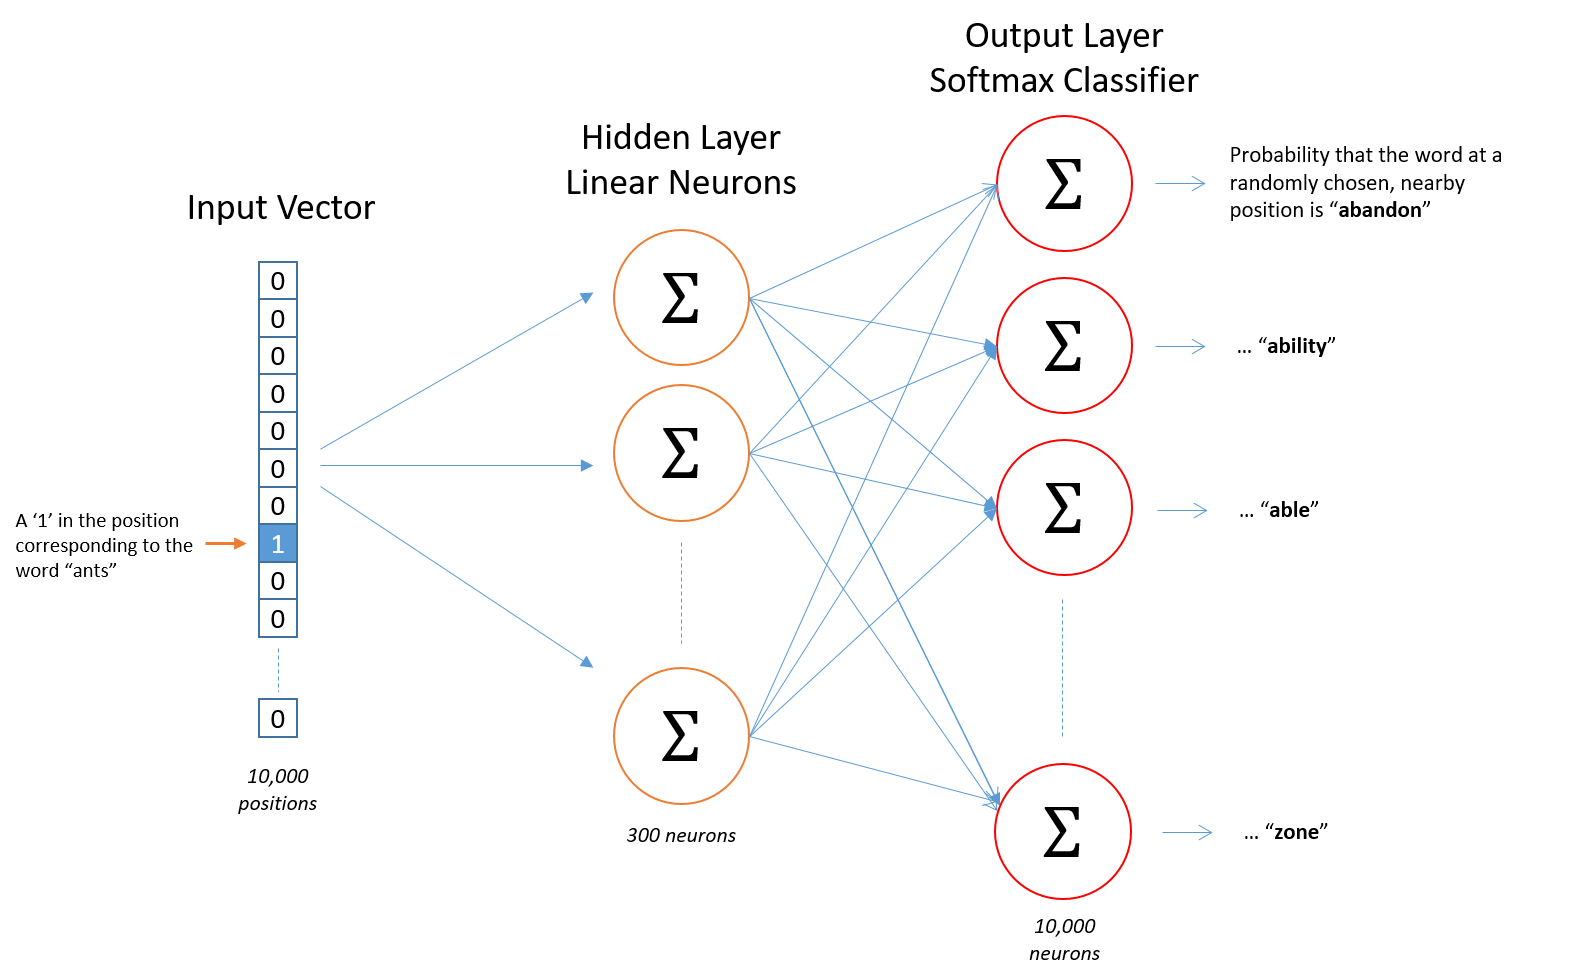
\includegraphics[width=\linewidth]{gfx/word2vec_arch}
	\caption[Architecture of a word2vec skip-gram model]{Example of a Skip-gram architecture. We can observe that $W = 10\,000$ and $n = 300$, meaning \emph{(a)} that the input vocabulary contains 10\,000 terms, and \emph{(b)} that for every word we wish to obtain a 300-dimensional vector representation. Here, the hyperparameter defining the window size is not shown.}
	\label{fig:skipgram}
\end{figure}

The input layer (also called \emph{projection layer}) receives words as a \emph{one hot encoded} vector, i.e. a vector of length $v$ where each element is equal to 0, except for the element whose position corresponds to the position of the input word in the vocabulary. If the vocabulary contains 10\,000 words, and the word ``ant'' appears in it at position 8, the input vector will contain all zeroes, and a single 1 in the 8th element.

A more formal definition of the Skip-gram model is as follows. Given a sequence of words $w_1, w_2, w_3, \dots, w_T$, i.e. the words in our vocabulary, the objective of the model is to maximize the average log probability, defined as:

\begin{equation} \label{eq:logprob}
\frac{1}{T} \sum\limits_{t=1}^{T}
\sum\limits_{-c \leq j \leq c, j \neq 0}
\log p(w_{t+j}|w_t)
\end{equation}
where $c$ is the window size. Skip-gram ideally defines $p(w_{t+j}|w_t)$ using a \emph{softmax} function:
\begin{equation} \label{eq:softmax}
p(w_O|w_I) = 
\frac
{\exp\left({\mathbf{v}'}_{w_O} {}^\mathsf{T} \mathbf{v}_{w_I}\right)}
{\sum\limits_{w=1}^{W}\exp\left({\mathbf{v}'}_w {}^\mathsf{T} \mathbf{v}_{w_I}\right)}
\end{equation}
where $\mathbf{v}_w$ and $\mathbf{v}'_w$ are the input and output vector representations of the word $w$, and $W$ is the number of words in the vocabulary.

However, this formulation is quite expensive, because its computing cost is proportional to the number $W$ of words in the vocabulary (which, in our case, we know to be around 300\,000). \citeauthor{mikolov2013efficient}, in order to approximate the full softmax\footnote{The first version of word2vec uses another approximation of the softmax, the \emph{hierarchical softmax}, not discussed here.}, propose a more efficient method, the \emph{negative sampling} (\acsfont{NEG}). \acsfont{NEG} is defined by the following objective function, which will replace every $\log P(w_O|w_I)$ term in \autoref{eq:logprob}:
\begin{equation} \label{eq:negsamp}
\log \sigma\left(\mathbf{v}'_{w_O} {}^\mathsf{T} \mathbf{v}_{w_I}\right) +
\sum\limits_{i=1}^k \mathbb{E}_{w_i \sim P_n(w)}
\left[\log \sigma\left(-\mathbf{v}'_{w_i} {}^\mathsf{T} \mathbf{v}_{w_I}\right)\right]
\end{equation}

Here, $\sigma(x) = 1 / (1 + \exp(-x))$. The task of this optimization is to distinguish the target word $w_O$ from random draws from the noise distribution $P_n(w)$ using logistic regression. The hyperparameter $k$ defines the \emph{negative samples}, or how many words from the noise distribution will be chosen to be ``distinguished'' from the target word $w_O$. The noise distribution $P_n(w)$ has been set by the authors as
$$
\frac{U(w)^{3/4}}{Z}
$$
where $U(w)$ is the \emph{unigram distribution}. The reported value in their experiments has been observed to outperform both the simple unigram distribution and the uniform distribution.

A perhaps more intuitive explanation of the Skip-gram architecture with negative sampling is the following. Whenever the model receives an input word $w_I$ as a one hot encoded vector $\mathbf{h}$, it retrieves from the projection layer the neuron $\mathbf{n}_i$, where $i$ is the index of the only element equal to 1 in $\mathbf{h}$ (the position of the word inside the vocabulary). This neuron holds the weights of the vector representation of $w_I$. Note that before the training starts, each neuron in the projection layer has to be initialized, usually with small random values.

In an ideal scenario (i.e., when using softmax, see \autoref{eq:softmax}), during training each vector representation of all the words $w_O$ in the vocabulary should either be ``pulled closer'' to $\mathbf{n}_i$ or ``pushed away'' from $\mathbf{n}_i$ by a small fraction, depending respectively on whether $w_O$ belongs to the context of $w_I$ or not. With negative sampling, however, the operation of ``pushing away'' the out-of-context word vectors is not performed for every word in the vocabulary, but only on a small subset randomly chosen from all of the out-of-context words.

There is a further optimization worth mentioning, due to the fact that it will affect data preprocessing. Raw textual sources contain a high number of words which do not carry much information, such as articles and prepositions. For example, if the model will benefit from observing the co-occurrence of the term ``guitarist'' with the term ``guitar'', it will benefit much less from observing the co-occurrence of the term ``the'' with the term ``guitarist'', since almost every word can co-occur frequently with ``the'' in a sentence. For this reason, Skip-gram subsamples frequent words according to the following equation:
\begin{equation}
P(w_i) = 1 - \sqrt{\frac{t}{f(w_i)}}
\end{equation}
meaning that each word $w_i$ in the training set will be discarded with a probability $P(w_i)$. The term $f(w_i)$ is the frequency of the word $w_i$, and $t$ is an arbitray threshold, set by the authors at around $10^{-5}$.

The advantages of adopting the Skip-gram model are several: 
\begin{itemize}
\item we can perform a \emph{streamed} type of training, meaning that less computational resources are needed since we won't have to keep all of the corpus loaded in memory all the time; in fact, we can feed the model with one sentence at a time, and then discard it when the next sentence comes in.
\item supposing the generated vector representations contain 300 elements each\footnote{This is an indicative value most people tend to suggest as an upper limit, after which overfitting will likely occur, but the choice of the vector size depends on the application.}, the output matrix computed on our vocabulary will only contain about 90 million entries, corresponding to 0.1\% of the size of what we would get by using simple co-occurrence matrices;
\item the amount of needed preprocessing is minimal, because, as we have seen, Skip-gram already contemplates a mechanism for discarding irrelevant terms; moreover, processes such as stemming\footnote{Stemming is the process of reducing inflected (or sometimes derived) words to their word stem, base or root form (e.g., the words ``beauty'', ``beautiful'' and ``beautifully'' share the same word stem ``beauti'').} and lemmatization\footnote{Lemmatization is the process of grouping together the inflected forms of a word so they can be analysed as a single item, identified by the word's lemma, or dictionary form (e.g., the words ``play'', ``plays'' and ``played'' share the same lemma ``play'').} become less relevant, because the model should implicitly figure out that terms sharing the same stem or lemma are in some way similar.
\end{itemize}

This said, the main reason supporting our choice of relying on this model is that the resulting vector representations will not only generate a semantic space where similar words end up close to each other, but they will be able to represent multiple degrees of similarity between words (\cite{mikolov2013linguistic}). For our purpose, and given the difficulties encountered in attributing to aesthetic terminology a universal meaning, we could maybe expect to observe one of two scenarios: words such as ``beauty'' or ``beautiful'' will \emph{(a)} be very similar to many different (musical) categories of terms (belonging to emotions, instruments, genres, \ldots), or \emph{(b)} live in a rather isolated corner of the output semantic space, distant from any specific/recognizable category of items.

\subsubsection{Preprocessing and training}
Before training the model, it is necessary to build the vocabulary we wish to represent. It has been said before that usually the vocabulary of a dataset is the collection of the single terms used in the documents; however, \citeauthor{mikolov2013efficient} suggest to include in the vocabulary idiomatic phrases whose meaning does not derive from a simple composition of the individual words -- what in technical language are referred to as \emph{n-grams}. Examples of music inspired n-grams would be ``electric guitar'', or ``hip hop'', or ``Guns'n'Roses''. Therefore, we first generated a list of n-grams (up to phrases of three words, or trigrams\footnote{N-grams can make the model more expressive, but they will also increase data sparsity, so we should be careful and use them with care.}) taken from our corpus that were added to the vocabulary.

Once we defined a vocabulary, we finally trained the Skip-gram model on a lowercased copy of the dataset. Lowercasing raw text is a common preprocessing step in \acsfont{NLP} tasks aimed at data cleaning (e.g., words appearing at the beginning of a sentence, or typos). The hyperparameters used in the training are reported in \autoref{tab:hyper}.
\begin{table}[t]
	\myfloatalign
	\begin{tabularx}{\textwidth}{lXc}
	\toprule
	\tableheadline{Parameter} & \tableheadline{Description} & \tableheadline{Value} \\
	\midrule
	size		& Size of each word's vector representations & 300 \\
	window 	& Maximum distance between the current word and the predicted context words within a sentence & 5 \\ 
	negative & Number of negative samples & 5 \\
	\bottomrule
	\end{tabularx}
	\caption{Hyperparameters of the word2vec Skip-gram model}
	\label{tab:hyper}
\end{table}

\section{Querying and clustering}\label{sec:query}
Any word embedding will generate a semantic space, a high-dimen\-sional projection of the vocabulary where every word is represented by vectors. These vectors can be seen as points occupying a specific position inside this multidimensional space. As such, we can apply standard clustering techniques to further describe the semantic space, and to characterize the similarities between words. If it is possible to succesfully cluster together words that appear to share a semantic connection, it means that there are good chances the embedding contains organized information, for which the clustering itself can provide some degree of explanation\footnote{In the next chapter, a less hand-wavy method for evaluating the quality of a word embedding will be introduced, along with results obtained on our dataset.}.

For this task, what we did was to query the Skip-gram model trained on our data with a list of ``aesthetic terms'', in order to obtain the closest words to each input query. This simple list comprises the following groups of words:
\begin{itemize}
	\item aesthetic -- aesthetics
	\item beautiful -- beautifully -- beauty
	\item ugliness -- ugly
\end{itemize}
which are very explicit terms related to aesthetics or to beauty (along with their antonyms, adjectives and adverbs).

We finally used a k-means algorithm to cluster the ``close terms'', or \emph{nearest neighbours}, returned from the model. The nearest neighbours of a word $w$ are all words $v \in V \setminus \left\{w\right\}$ (where $V$ is the vocabulary) sorted in descending order by $\text{similarity}(w,v)$; the similarity, again, is defined by the cosine distance between vector representations of $w$ and $v$ (see \autoref{eq:cossim}). By doing so we tried to identify semantic classes of word clusters that could reasonably answer our question: what do people refer to when they argue over musical beauty?

\section{Final note}
All the code and the data used in the steps reported here and in the next chapter are open-source and accessible at the following link:
\begin{quote}
	\url{https://github.com/lorenzo-romanelli/compbeauty_code}
\end{quote}

























\cleardoublepage
\chapter{Results}\label{ch:results}
In this chapter, we will mainly present the results obtained on our dataset by following the methodology previously discussed. Before doing so, however, we feel like a brief discussion on quality evaluation of word embeddings is necessary.

\section{Evaluation of word embeddings}
Techniques such as word2vec are powerful tools for representing meaning using geometry. As with any model working on real data, it is important to conduct a rigorous evaluation which can justify its goodness. Our scenario makes no exception, especially given the exploratory nature of the task we are after. Relying so much on this model to explore the dataset while looking for meaningful semantic relationships means we must be sure that the model actually learned these relationships.

Good overviews of evaluation methods for word embeddings can be found in \cite{schnabel2015evaluation} and \cite{bakarov2018survey}. The reason why there exist many evaluation methods can be reconduced to the instrinsic difficulty in determining semantic similarity/relatedness in a broader sense. If we add to that that words have multiple degrees of similarity, that the structure of embeddings can greatly vary across corpora and models, and that, in general, there is a lack of correlation between different performance scores, the challenges of choosing or designing a meaningful evaluation system become even more evident. 

There are two evaluation methods we find to be the most suitable here. The first is based on \emph{Gold Standard Corpora} (\acsfont{GSC}), lists compiled by hand by linguists or field experts where pairs of words are given an explicit similarity score. These lists are then compared with the model, and an aggregated estimate is calculated (usually, Pearson or Spearman correlation coefficient). Such an estimate reports the similarity of semantic relationships as inferred by the embedding to the semantic relationships as inferred by human experts. The advantage of adopting \acsfont{GSC} is that they can be compiled to be quite domain-specific; specificity is useful to disambiguate, for example, cases of polysemy (words with more than one meaning) and in general helps to restrict semantic judgments to the domain the model is supposed to work in\footnote{For example, \cite{sugathadasa2017synergistic} demonstrated the usefulness of using domain-specific \acsfont{GSC} to evaluate embeddings trained on legal documents.}. 

We are working in the music domain; for this reason, we looked for openly available \acsfont{GSC} to evaluate our model, without success. Unfortunately, as \cite{wissler2014gold} observe, building a \acsfont{GSC} manually results in a costly process, both in terms of time and resources. This prevented us from creating our own evaluation corpus here, but we hope this gap can be filled as soon as possible.

The second evaluation method taken into consideration is somehow similar to the one just discussed, with two main differences:
\begin{enumerate}
\item the lists are not domain-specific, but can span rather general contexts;
\item the lists are based on judgments of people who do not necessarily have a background in Linguistics.
\end{enumerate}
The advantage of using such lists over \acsfont{GSC} is that the former are more widely available. The drawback is that, when comparing their content with domain-specific datasets such as ours, the model's goodness can suffer from being tested on words not belonging or marginal to that specific context.

\subsection{Evaluating our model}\label{subsec:eval}
What has been described in the last paragraph is exactly what happened to us. We decided to adopt a standard list, the \emph{wordsim353}\footnote{Introduced in \cite{finkelstein2001placing} and available at \url{http://alfonseca.org/eng/research/wordsim353.html}}, and we tested our embedding with it. The aggregated estimate yielded a Spearman's rank correlation coefficient of 0.45 ($p$ $<$ 0.05). However, almost 60\% of the tuples in the list could not be evaluated, because they featured terms which did not appear at all in our corpus.

Previous results thus demand other ways of assessing the quality of our embedding. Having to deal with music, we proceeded with more empirical explorations of the model, looking for meaningful musical semantic relationships. Taking inspiration from \cite{mikolov2013distributed}, where the authors observed how their model could implicitly learn and organize concepts such as countries and capitals and their association, we explored whether our embedding could discriminate between \emph{musicians} and their relative \emph{instruments}.

\autoref{fig:player-instr} shows the result of this exploration. It is interesting to observe not only how the model learned to discriminate between the concept of musician and the concept of musical instrument, but also how it almost mantained the same hierarchy between musicians and instruments (except for the drummer-drums pair). Terms traditionally associated with rock-type of genres appear towards the bottom, whereas moving towards the top part of the plot more classic instruments/musicians appear. The voice-singer pair appears in a more distant corner, likely due to the polysemous nature of the term \emph{voice} and to the fact that voice cannot be properly defined as an instrument.

\begin{figure}[bth]
	\myfloatalign
	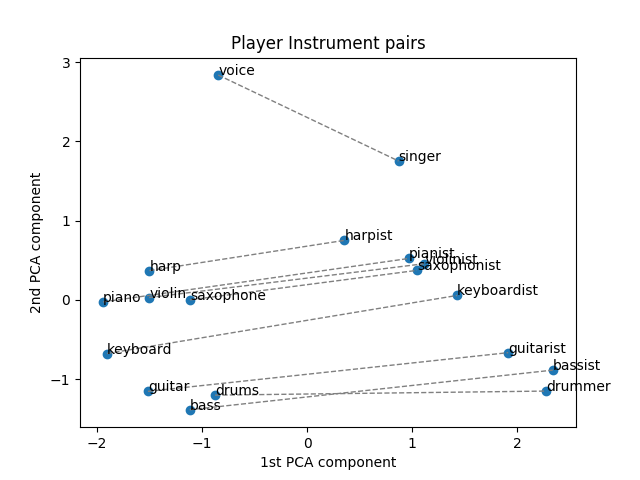
\includegraphics[width=\linewidth]{gfx/player-instrument2}
	\caption[\acsfont{PCA} plot of player-instrument word pairs]{Plot of a \acsfont{PCA} with 2 components performed on word vectors for pairs of musicians-played instrument. The model has succesfully learned the difference between these two classes of musical concepts (instruments on the left, musicians on the right).}
	\label{fig:player-instr}
\end{figure}

Next, we briefly explored how the model organized music genres. A \acsfont{PCA} plot of a list of music genres words is shown in \autoref{fig:genres}. What the model seems to have learned is interesting. On the far left-side of the graph we find more rhythm-driven genres (rap, hip-hop, dance, techno, house), while all the genres towards the bottom seem to have in common their black origins. Classical music, opera and religious appear on the top-right, while rock, metal, pop and alternative live towards the center of the plot. On the far right-side are featured typical traditional American genres, such as bluegrass, folk, country, gospel and blues.

\begin{figure}[tp]
	\myfloatalign
	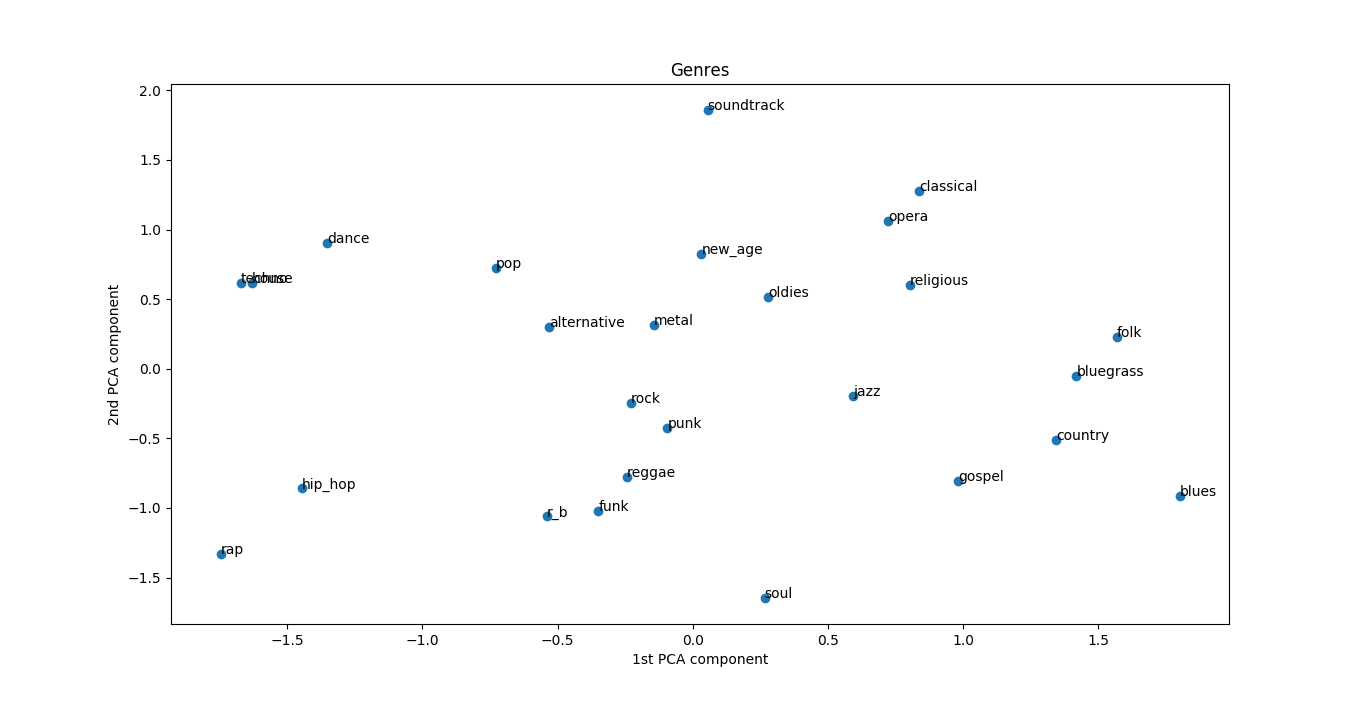
\includegraphics[angle=-90,origin=c,width=\linewidth]{gfx/genres}
	\caption[\acsfont{PCA} plot of music genres words]{Plot of a \acsfont{PCA} with 2 components performed on word vectors for music genres.}
	\label{fig:genres}
\end{figure}

These are just two examples of some empirical observations we made on our dataset regarding musical concepts. While it is true that no rigorous evaluation confirmed how reliable the model effectively is, the plots shown above give us enough confidence that the model can represent music-related concepts with a reasonable degree of semantic organization. For sure, when more proper evaluation techniques will be avaliable for this type of data, it will be advisable for us to provide a more grounded justification of our embedding.

\section{Results}
\subsection{Nearest neighbours}\label{subsec:nearest}
For each of the aesthetic terms listed in \autoref{sec:query}, we first queried our model for the 10 words which appeared closer to the input, in terms of cosine similarity between their vector representations. 

The 10 closest words returned by the model for the words \emph{beauty--beautiful--beautifully} are reported in \autoref{tab:beauty10nearest}. The first interesting result is that for \emph{beauty} and \emph{beautifully}, all of the top 10 nearest words are nouns and adverbs, respectively, just like the query words, whereas for \emph{beautiful} not only adjectives are retrieved, but also some adverbs (\emph{achingly} and \emph{crushingly}). For all of three words, there is no term living notably close to the respective query word (if this was the case, there would be semantic equivalence), since all of the cosine similarities are below 0.7. Third, there are very few words referring to concrete objects or qualities; abstract concepts seem to be dominant.

\begin{table}[tbh]
\myfloatalign
\small
\begin{tabular}{ll}
\toprule
\multicolumn{2}{c}{beauty}\\ \midrule
	ugliness & 0.6402 \\
	serenity & 0.6355 \\
	loveliness & 0.6252 \\
	listlessness & 0.6197 \\
	sublimity & 0.6191 \\
	prettiness & 0.6159 \\
	quietude & 0.6155 \\
	fragility & 0.6143 \\
	elegance & 0.6049 \\
	imperfection & 0.5943 \\
	\bottomrule
\end{tabular}
\begin{tabular}{ll}
\toprule
\multicolumn{2}{c}{beautiful}\\ \midrule
	gorgeous & 0.6994 \\
	lovely & 0.6354 \\
	transfixing & 0.623 \\
	achingly & 0.6195 \\
	wonderful & 0.6195 \\
	crushingly & 0.6173 \\
	stunning & 0.6089 \\
	affecting & 0.6042 \\
	spellbinding & 0.6042 \\
	beguiling & 0.602 \\
	\bottomrule
\end{tabular}
\begin{tabular}{ll}
\toprule
\multicolumn{2}{c}{beautifully}\\ \midrule
	exquisitely & 0.6669 \\
	gorgeously & 0.6542 \\
	sumptuously & 0.6523\\ 
	flawlessly & 0.6452\\
	pristinely & 0.6288\\
	thoughtfully & 0.6242\\
	marvelously & 0.6166\\
	impeccably & 0.6144 \\
	elegantly & 0.6124\\
	superbly & 0.5948\\
\bottomrule
\end{tabular}
\caption[Nearest neighbours for \emph{beauty-beautiful-beautifully}]{Top 10 nearest neighbours for the words \emph{beauty--beautiful--beautifully}. Left column reports the word, right column the cosine similarity.}
\label{tab:beauty10nearest}
\end{table}

\autoref{tab:aesth10nearest} reports the 10 closest words returned by the model for the words \emph{aesthetic--aesthetics}. It is more challenging to give an interpretation of the semantic relationships in these results. \emph{Aesthetics} appears to be associated to concepts bound to tradition, universalism and timelessness, conveying images of something that is there and should not be questioned (\emph{tenets}; \emph{paradigms}; \emph{conversant}; \emph{vocabularies}; \emph{idioms}; \emph{forbears}). This idea partly returns for \emph{aesthetic}, but here the concepts seem to have a more abstract acception, which can be subject to personal attitude and interpretation (\emph{worldview}; \emph{ethos}; \emph{principles}; \emph{approach}).

\begin{table}[bth]
\myfloatalign
\small
\begin{tabular}{ll}
\toprule
\multicolumn{2}{c}{aesthetic}\\ \midrule
worldview & 0.5978\\
purview & 0.5902\\
aesthetics & 0.5875\\
ethos & 0.5819\\
principles & 0.5768\\
approach & 0.5758\\
alchemical & 0.5756\\
plasticity & 0.5729\\
perfectionism & 0.5672\\
frameworks & 0.5664\\
\bottomrule
\end{tabular}
\begin{tabular}{ll}
\toprule
\multicolumn{2}{c}{aesthetics}\\ \midrule
tenets & 0.6536\\
affinities & 0.653\\
paradigms & 0.652\\
synthesists & 0.6382\\
conversant & 0.6332\\
bastardizing & 0.633\\
vocabularies & 0.6316\\
idioms & 0.6286\\
hybridization & 0.6231\\
forbears & 0.6219\\
\bottomrule
\end{tabular}
\caption[Nearest neighbours for \emph{aesthetic-aesthetics}]{Top 10 nearest neighbours for the words \emph{aesthetic--aesthetics}.}
\label{tab:aesth10nearest}
\end{table}

Finally, in \autoref{tab:ugly10nearest} the resulting nearest neighbours for \emph{ugliness--ugly} have been reported. \emph{Ugliness}, up to now, is the only term whose cosine similarities with retrieved neighbours are almost all above 0.7. It is interesting to observe how words close to it do not necessarily possess a negative connotation (\emph{placidity}; \emph{exhilaration}; \emph{surreality}). The same cannot be said for \emph{ugly}: almost the totality of its neighbours have a very negative polarity, except for the first two (\emph{casanova}; \emph{ugly})\footnote{This very last observation is easily explained: \emph{Ugly Casanova} and \emph{Ugly Duckling} are the names of two bands.}.

\begin{table}[bth]
\myfloatalign
\small
\begin{tabular}{ll}
\toprule
\multicolumn{2}{c}{ugliness}\\ \midrule
placidity & 0.7308\\
messiness & 0.7307\\
discord & 0.7254\\
exhilaration & 0.7229\\
surreality & 0.71\\
discomfort & 0.7088\\
nakedness & 0.701\\
listlessness & 0.7005\\
eeriness & 0.6969\\
bleakness & 0.695\\
\bottomrule
\end{tabular}
\begin{tabular}{ll}
\toprule
\multicolumn{2}{c}{ugly}\\ \midrule
casanova & 0.6006 \\
duckling & 0.5876\\
angry & 0.5732\\
vulgar & 0.5352\\
inappropriately & 0.5347\\
unrelentingly & 0.5328\\
repellant & 0.5265\\
unrepentantly & 0.5259\\
disgusting & 0.5222\\
exasperating & 0.5201\\
\bottomrule
\end{tabular}
\caption[Nearest neighbours for \emph{ugly-ugliness}]{Top 10 nearest neighbours for the words \emph{ugly--ugliness}.}
\label{tab:ugly10nearest}
\end{table}

\subsection{Clustering}
The results presented up to now hint at some patterns in the way our model organizes both musical and aesthetic information. Here we tried to cluster the 100 nearest neighbours to each aesthetic term using a k-means strategy. Since k-means should be provided with the number of clusters the algorithm has to compute (parameter $k$), we ran different analyses varying $k$ and evaluating eacht time the output.

Unfortunately, our quest looking for meaningful word clusters was not particularly successful. Clusters generated in this way look messy, as they include set of words for which finding a common semantic thread is difficult. As an example, we provide the clusters generated for the term \emph{beauty}, with $k$ $=$ 7, in \autoref{tab:clus}. Clusters computed on the other words of our list and with other values for $k$ have been omitted, since they all more or less follow the same pattern -- or, better said, \emph{non}-pattern. 

As we can see, there is a dominating cluster (cluster \#3) containing a big amount of terms which do not appear to have much in common with each other. There are clusters made of only one word, while clusters \#1, \#6 and \#7, which are neither too big or too small, still appear to have been built arbitrarily. Increasing the value of $k$ to try to ``break down'' in more meaningful chunks overly sized clusters, such as cluster \#3 here, has had the only effect of generating a higher number of small clusters containing only one or two words.

\begin{table}[t]
\myfloatalign
\small
\begin{tabularx}{\textwidth}{lX}
\toprule
\acsfont{cluster 1} & prettiness, brightness, delicacy, richness \\
\acsfont{cluster 2} & majesty \\
\acsfont{cluster 3} & listlessness, sublimity, quietude, gorgeousness, gentleness, melancholia, hopefulness, steadiness, discord, undisturbed, eeriness, combustion, peacefulness, bittersweetness, togetherness, coldness, aggressiveness, otherworldliness, pensiveness, nourishment, sakura, placidity, necessities, wrongness, greenery, shroud, insoluble, stateliness, frailty, bleakness, circularity, mutability, solemnity, pleasantness, crispness, clumsiness, ominousness, attains, nakedness, humankind, incompleteness, cultivation, ethereality, disquietingly, solidity, softness, impenetrability, chilliness, unhampered, remoteness, soulfulness, engravings, resourcefulness, jubilance, disquiet, apprehension, manmade, malevolence, splendor, precariousness, enormity, disconnection, wonderment, peril, carnality, trimmings, commotion, vibrancy, engulfing, expansiveness, symbiosis \\
\acsfont{cluster 4} & warmth \\
\acsfont{cluster 5} & sadness \\
\acsfont{cluster 6} & ugliness, serenity, contemplation, elation, exhilaration, vulnerability, pessimism, disorientation, tranquility, uneasiness \\
\acsfont{cluster 7} & loveliness, fragility, elegance, imperfection, poignancy, strangeness, transparency, messiness, lucidity, eloquence, intrigue, persistence \\
\bottomrule
\end{tabularx}
\caption{K-means clustering on the nearest neighbours of the word \emph{beauty}}
\label{tab:clus}
\end{table}

In our opinion, there could be three explanations for this behaviour. First, the model could have failed to learn a meaningful representation of semantic relationships between abstract terminology. Abstractness, in fact, seems to be almost the only thread connecting the reported data. This would in part disprove the observations reported in \autoref{subsec:nearest}. Second, the intrinsic difficulties of defining aesthetic terms could have had the effect of projecting them in corners of the word embedding at the intersection of many different semantic areas. This would make it impossible to find common conjunction points between these areas. Third, the model could simply be overfit on the data. If this was the case, the vector representations of words would almost become like one hot vectors, every one living independently from the others without any connection. This however would disprove many of the things we observed in \autoref{subsec:eval}.

\section{Google News dataset}
Finally, we decided to perform a similar analysis on a different model. This model is not trained on specific music-related data, and was provided by \citeauthor{mikolov2013distributed} as part of their research\footnote{\url{https://drive.google.com/file/d/0B7XkCwpI5KDYNlNUTTlSS21pQmM/}}. The training has been carried out on a dataset of about 100 billion words coming from a huge collection of Google News articles, using a Skip-gram architecture with negative sampling. Generated word vectors have 300 dimensions, while the size of the vocabulary has been cut down by us to the first 500\,000 words, according to their frequency in the corpus (only the most frequent have been kept).

In this scenario, our clustering attempts have proven to be much more successful. We have queried the model for the 500 nearest neighbours\footnote{This number has been chosen instead of 100 for two reasons: \emph{(a)} this dataset is much bigger in size and scope, thus potentially including many more concepts related to beauty other than music; \emph{(b)} the authors did not lowercase the dataset before training, which means that, for example, both \emph{beautiful} and \emph{BEAUTIFUL} are included in the vocabulary.}, and clustered them using k-means. The results for the term \emph{beauty} setting $k$ $=$ 15 are shown in \autoref{tab:gbeauty} (results have been cut down to ten words per cluster). The first thing that jumps to the eye is how much the quality of the clusters improves. All of the clusters contain semantically related words, or words belonging to a common topic. It is also noticeable how much more concrete the concept of beauty appears to be in a general context; many are the references to femininity, sensuality, cosmetics, personal grooming, but also to nature, flowers, architecture. Sadly, not much appears about arts and music.

\begin{table}[tp]
\myfloatalign
\small
\begin{tabularx}{\textwidth}{lX}
\toprule
\multicolumn{2}{c}{beauty} \\
\midrule
\acsfont{cluster 1} & Beauty, skincare, cosmetics, Natural\_Beauty, haircare, Pantene, Shu\_Uemura, Aveda, Lancome, Cosmetics, ... \\
\acsfont{cluster 2} & esthetics, aesthetic, aesthetics, artistry, esthetic, visual\_splendor, artifice, intricacy, originality, starkness, ... \\
\acsfont{cluster 3} & scenic\_beauty, beautiful\_scenery, sweeping\_vistas, breathtakingly\_beautiful, landscapes, splendours, scenery, gorgeous\_scenery, sceneries, picturesque\_scenery, ... \\
\acsfont{cluster 4} & lip\_balms, shampoos\_conditioners, paraben\_free, Body\_Wash, lip\_glosses, aging\_creams, skin\_whitening, shower\_gels, cosmeceuticals, cosmeceutical, ...
 \\
\acsfont{cluster 5} & eyelash\_extensions, estheticians, cosmetic, stylist, hair\_styling, salon, hair\_extensions, esthetician, false\_eyelashes, Makeup, ...\\
\acsfont{cluster 6} & loveliness, magnificence, splendor, serenity, grandeur, majesty, sensual\_pleasures, splendors, sublimity, tranquility, ... \\
\acsfont{cluster 7} & lingerie, Glamour, bridal, fashion, sexy\_lingerie, Allure, beachwear, boho\_chic, StyleList, bridal\_boutique, ... \\
\acsfont{cluster 8} & glamor, gorgeousness, sexiness, pulchritude, fabulousness, classiness, va\_va\_voom, je\_ne\_sais\_quoi, sparkle, tackiness, ... \\
\acsfont{cluster 9} & radiance, naturalness, uniqueness, prettiness, allure, sensuality, timelessness, exoticism, sensuousness, pureness, ... \\
\acsfont{cluster 10} & beauties, plumpness, curvaceous, feminine, curvy, womanly, voluptuous, supermodel, hourglass\_figure, glamorously, ... \\
\acsfont{cluster 11} & PURE\_ranges, fragrance, proto\_col, BEAUTY, perfume, essences, On\_Group.co.uk\_manufacture, handcrafted\_jewelry, floral, Lush, ... \\
\acsfont{cluster 12} & beautiful, gorgeous, ethereal\_beauty, ravishing, sensual, luscious, fabulous, stunningly\_beautiful, sensuous, alluring, ... \\
\acsfont{cluster 13} & elegance, rustic\_charm, timeless\_elegance, opulence, interior\_decor, décor, understated\_elegance, decor, luxe, craftsmanship, ... \\
\acsfont{cluster 14} & spa, spas, aromatherapy, luxurious\_spa, pampering, pamper\_yourself, Aromatherapy, manicure\_pedicure, Spa, Spas, ... \\
\acsfont{cluster 15} & femininity, womanhood, individuality, ordinariness, preciousness, specialness, aliveness, spirituality, wholeness, intimacy, ...\\
\bottomrule
\end{tabularx}
\caption{K-means clustering on the nearest neighbours of the word \emph{beauty} (Google News dataset)}
\label{tab:gbeauty}
\end{table}

As a final point, in \autoref{tab:gbfully} is reported one of the clusters that showed up while exploring the neighbours of \emph{beautifully} in this model. It is evident why it caught our attention: this is the most fulgid example, up to now, of real, tangible musical features that people might be addressing when talking about beauty in music.

\begin{table}
\myfloatalign
\small
\begin{tabularx}{\textwidth}{X}
\toprule
beautifully\_sung, recitatives, vocalism, harmonically, orchestral\_accompaniment, rhythmically, lyricism, rhythmical, melodically, cadenzas, contrapuntal, tonalities, sonority, acoustically, pizzicato, sonorities, Tyagaraja, rhythmic\_patterns, legato, fugues, expressivity \\
\bottomrule
\end{tabularx}
\caption{Cluster extracted from the neighbours of the word \emph{beautifully} (Google dataset)}
\label{tab:gbfully}
\end{table}

\cleardoublepage
\chapter{Conclusions}\label{ch:conclusion}
\section{Summary}
With this work, we aimed at outlining a new approach to the study of beauty from a computational perspective, as well as an introductory exploratory study on music reviews. We began by questioning whether is it possible to attribute objective, universal characteristics to musical aesthetic experiences. As we provided an overview of existing aesthetic theories and studies grounded in philosophy, cognitive neurosciences and computer science, it soon became evident how we are indeed facing a much bigger task. Our state of the art review, in fact, surfaced the problem of providing universally accepted definitions of the concept of beauty. What emerged was the need of addressing this problem from another perspective, a perspective grounded on aesthetic judgments addressed in real-life scenarios. Such scenarios constitute those situations where people explicitly talk about beauty by relating it to actual features of objects, which make possible their practical study.

\section{Discussion}
This project started as an attempt to build a computational model able to extract concrete musical features related to beauty from a corpus of music reviews. It was an ambitious goal, and in fact our analyses turned out to provide satisfying results only in part. Using word embeddings to model semantic spaces is a well-established procedure in \acsfont{NLP} applications; extracting information from such embeddings, instead, is not that easy.

The main roadblock here has been the blurry interpretability of the semantic relationships learned by the model, due to a number of possible reasons. We tried to identify some shortcomings with our experiments, namely:
\begin{itemize}
\item lack of proper sources and methodologies to evaluate the model;
\item lack of enough training data;
\item overfitting.
\end{itemize}

These conclusions were drawn after applying the same methodology we adopted on our music reviews dataset to a much bigger, general purpose set of documents. In this scenario, we were able to spot much more meaningful relationships, with a hint at concrete musical features that should be further investigated. This gives us good reasons to believe that our proposed approach has potential, both conceptually and practically. We do hope that our research efforts can be further developed.

\section{Future work}
What has been presented here is only a starting point towards developing a comprehensive study of beauty, in music and not, grounded in language and aided by artificial intelligence. Of course our model can and has to be improved, evaluated and expanded. Once again, the Internet is the most valuable source for this task. Many well respected online music magazines exist, and scraping the required information from them can significally increase the size and the quality of the dataset. Also, more robust strategies for extracting explicit semantic relationships in word embeddings should be investigated.

Good starting points for this task would be semantic or lexical networks such as WordNet\footnote{\url{https://wordnet.princeton.edu/}} or ConceptNet\footnote{\url{http://conceptnet.io/}}. These are graphs whose nodes represent terms or phrases in natural language, while edges connect them using explicit semantic relationships (like \emph{is-a}, \emph{similar-to}, \emph{part-of}, \emph{synonym}, \emph{antonym}, and so on). By exploiting such graphs, we could for example develop a semantic-based clustering strategy.

If the proposed (or similar) methodologies prove to be successful, many different studies could be carried on. Some ideas include a comparison of the semantic changes of aesthetic terms in music across time periods, different cultures, or music genres.

The most interesting application these studies can find is probably to use them in synergy with research coming from other fields. One could think about developing systems which make use of prescriptive lists of features extracted from experts' opinions about beauty and apply them to actual pieces of music. By doing so we could for example provide a concrete support to the work of musicologists and musicians, as well as further pushing forward our knowledge about judgments of beauty in all of its many facets: subjective or objective, conscious or subconscious, universal or particular.

%\ctparttext{You can put some informational part preamble text here.
%Illo principalmente su nos. Non message \emph{occidental} angloromanic
%da. Debitas effortio simplificate sia se, auxiliar summarios da que,
%se avantiate publicationes via. Pan in terra summarios, capital
%interlingua se que. Al via multo esser specimen, campo responder que
%da. Le usate medical addresses pro, europa origine sanctificate nos se.}
%\part{The Showcase}\label{pt:showcase}
%\include{Chapters/Chapter02}
%\addtocontents{toc}{\protect\clearpage} % <--- just debug stuff, ignore
%\include{Chapters/Chapter03}
%\include{multiToC} % <--- just debug stuff, ignore for your documents
% ********************************************************************
% Backmatter
%*******************************************************
%\appendix
%\renewcommand{\thechapter}{\alph{chapter}}
%\cleardoublepage
%\part{Appendix}
%\include{Chapters/Chapter0A}
%********************************************************************
% Other Stuff in the Back
%*******************************************************
\cleardoublepage%********************************************************************
% Bibliography
%*******************************************************
% work-around to have small caps also here in the headline
% https://tex.stackexchange.com/questions/188126/wrong-header-in-bibliography-classicthesis
% Thanks to Enrico Gregorio
\defbibheading{bibintoc}[\bibname]{%
  \phantomsection
  \manualmark
  \markboth{\spacedlowsmallcaps{#1}}{\spacedlowsmallcaps{#1}}%
  \addtocontents{toc}{\protect\vspace{\beforebibskip}}%
  \addcontentsline{toc}{chapter}{\tocEntry{#1}}%
  \chapter*{#1}%
}
\printbibliography[heading=bibintoc]

% Old version, will be removed later
% work-around to have small caps also here in the headline
%\manualmark
%\markboth{\spacedlowsmallcaps{\bibname}}{\spacedlowsmallcaps{\bibname}} % work-around to have small caps also
%\phantomsection
%\refstepcounter{dummy}
%\addtocontents{toc}{\protect\vspace{\beforebibskip}} % to have the bib a bit from the rest in the toc
%\addcontentsline{toc}{chapter}{\tocEntry{\bibname}}
%\label{app:bibliography}
%\printbibliography

%\cleardoublepage\include{FrontBackmatter/Declaration}
%\cleardoublepage\pagestyle{empty}

\hfill

\vfill


\pdfbookmark[0]{Colophon}{colophon}
\section*{Colophon}
This document was typeset using the typographical look-and-feel \texttt{classicthesis} developed by Andr\'e Miede and Ivo Pletikosić.
The style was inspired by Robert Bringhurst's seminal book on typography ``\emph{The Elements of Typographic Style}''.
\texttt{classicthesis} is available for both \LaTeX\ and \mLyX:
\begin{center}
\url{https://bitbucket.org/amiede/classicthesis/}
\end{center}
Happy users of \texttt{classicthesis} usually send a real postcard to the author, a collection of postcards received so far is featured here:
\begin{center}
\url{http://postcards.miede.de/}
\end{center}
Thank you very much for your feedback and contribution.

\bigskip

\noindent\finalVersionString

%Hermann Zapf's \emph{Palatino} and \emph{Euler} type faces (Type~1 PostScript fonts \emph{URW
%Palladio L} and \emph{FPL}) are used. The ``typewriter'' text is typeset in \emph{Bera Mono},
%originally developed by Bitstream, Inc. as ``Bitstream Vera''. (Type~1 PostScript fonts were made
%available by Malte Rosenau and
%Ulrich Dirr.)

%\paragraph{note:} The custom size of the textblock was calculated
%using the directions given by Mr. Bringhurst (pages 26--29 and
%175/176). 10~pt Palatino needs  133.21~pt for the string
%``abcdefghijklmnopqrstuvwxyz''. This yields a good line length between
%24--26~pc (288--312~pt). Using a ``\emph{double square textblock}''
%with a 1:2 ratio this results in a textblock of 312:624~pt (which
%includes the headline in this design). A good alternative would be the
%``\emph{golden section textblock}'' with a ratio of 1:1.62, here
%312:505.44~pt. For comparison, \texttt{DIV9} of the \texttt{typearea}
%package results in a line length of 389~pt (32.4~pc), which is by far
%too long. However, this information will only be of interest for
%hardcore pseudo-typographers like me.%
%
%To make your own calculations, use the following commands and look up
%the corresponding lengths in the book:
%\begin{verbatim}
%    \settowidth{\abcd}{abcdefghijklmnopqrstuvwxyz}
%    \the\abcd\ % prints the value of the length
%\end{verbatim}
%Please see the file \texttt{classicthesis.sty} for some precalculated
%values for Palatino and Minion.
%
%    \settowidth{\abcd}{abcdefghijklmnopqrstuvwxyz}
%    \the\abcd\ % prints the value of the length

% ********************************************************************
% Game Over: Restore, Restart, or Quit?
%*******************************************************
\end{document}
% ********************************************************************
